% Options for packages loaded elsewhere
\PassOptionsToPackage{unicode}{hyperref}
\PassOptionsToPackage{hyphens}{url}
\PassOptionsToPackage{dvipsnames,svgnames,x11names}{xcolor}
%
\documentclass[
  authoryear,
  preprint,
  3p]{elsarticle}

\usepackage{amsmath,amssymb}
\usepackage{iftex}
\ifPDFTeX
  \usepackage[T1]{fontenc}
  \usepackage[utf8]{inputenc}
  \usepackage{textcomp} % provide euro and other symbols
\else % if luatex or xetex
  \usepackage{unicode-math}
  \defaultfontfeatures{Scale=MatchLowercase}
  \defaultfontfeatures[\rmfamily]{Ligatures=TeX,Scale=1}
\fi
\usepackage{lmodern}
\ifPDFTeX\else  
    % xetex/luatex font selection
\fi
% Use upquote if available, for straight quotes in verbatim environments
\IfFileExists{upquote.sty}{\usepackage{upquote}}{}
\IfFileExists{microtype.sty}{% use microtype if available
  \usepackage[]{microtype}
  \UseMicrotypeSet[protrusion]{basicmath} % disable protrusion for tt fonts
}{}
\makeatletter
\@ifundefined{KOMAClassName}{% if non-KOMA class
  \IfFileExists{parskip.sty}{%
    \usepackage{parskip}
  }{% else
    \setlength{\parindent}{0pt}
    \setlength{\parskip}{6pt plus 2pt minus 1pt}}
}{% if KOMA class
  \KOMAoptions{parskip=half}}
\makeatother
\usepackage{xcolor}
\setlength{\emergencystretch}{3em} % prevent overfull lines
\setcounter{secnumdepth}{5}
% Make \paragraph and \subparagraph free-standing
\ifx\paragraph\undefined\else
  \let\oldparagraph\paragraph
  \renewcommand{\paragraph}[1]{\oldparagraph{#1}\mbox{}}
\fi
\ifx\subparagraph\undefined\else
  \let\oldsubparagraph\subparagraph
  \renewcommand{\subparagraph}[1]{\oldsubparagraph{#1}\mbox{}}
\fi


\providecommand{\tightlist}{%
  \setlength{\itemsep}{0pt}\setlength{\parskip}{0pt}}\usepackage{longtable,booktabs,array}
\usepackage{calc} % for calculating minipage widths
% Correct order of tables after \paragraph or \subparagraph
\usepackage{etoolbox}
\makeatletter
\patchcmd\longtable{\par}{\if@noskipsec\mbox{}\fi\par}{}{}
\makeatother
% Allow footnotes in longtable head/foot
\IfFileExists{footnotehyper.sty}{\usepackage{footnotehyper}}{\usepackage{footnote}}
\makesavenoteenv{longtable}
\usepackage{graphicx}
\makeatletter
\def\maxwidth{\ifdim\Gin@nat@width>\linewidth\linewidth\else\Gin@nat@width\fi}
\def\maxheight{\ifdim\Gin@nat@height>\textheight\textheight\else\Gin@nat@height\fi}
\makeatother
% Scale images if necessary, so that they will not overflow the page
% margins by default, and it is still possible to overwrite the defaults
% using explicit options in \includegraphics[width, height, ...]{}
\setkeys{Gin}{width=\maxwidth,height=\maxheight,keepaspectratio}
% Set default figure placement to htbp
\makeatletter
\def\fps@figure{htbp}
\makeatother

\makeatletter
\@ifpackageloaded{caption}{}{\usepackage{caption}}
\AtBeginDocument{%
\ifdefined\contentsname
  \renewcommand*\contentsname{Table of contents}
\else
  \newcommand\contentsname{Table of contents}
\fi
\ifdefined\listfigurename
  \renewcommand*\listfigurename{List of Figures}
\else
  \newcommand\listfigurename{List of Figures}
\fi
\ifdefined\listtablename
  \renewcommand*\listtablename{List of Tables}
\else
  \newcommand\listtablename{List of Tables}
\fi
\ifdefined\figurename
  \renewcommand*\figurename{Figure}
\else
  \newcommand\figurename{Figure}
\fi
\ifdefined\tablename
  \renewcommand*\tablename{Table}
\else
  \newcommand\tablename{Table}
\fi
}
\@ifpackageloaded{float}{}{\usepackage{float}}
\floatstyle{ruled}
\@ifundefined{c@chapter}{\newfloat{codelisting}{h}{lop}}{\newfloat{codelisting}{h}{lop}[chapter]}
\floatname{codelisting}{Listing}
\newcommand*\listoflistings{\listof{codelisting}{List of Listings}}
\makeatother
\makeatletter
\makeatother
\makeatletter
\@ifpackageloaded{caption}{}{\usepackage{caption}}
\@ifpackageloaded{subcaption}{}{\usepackage{subcaption}}
\makeatother
\journal{Palaeo3}
\ifLuaTeX
  \usepackage{selnolig}  % disable illegal ligatures
\fi
\usepackage[]{natbib}
\bibliographystyle{elsarticle-harv}
\usepackage{bookmark}

\IfFileExists{xurl.sty}{\usepackage{xurl}}{} % add URL line breaks if available
\urlstyle{same} % disable monospaced font for URLs
\hypersetup{
  pdftitle={Confirmation of Mg/Ca ratios as palaeothermometers in Atlantic limpet shells},
  pdfauthor={Niklas Hausmann; Donna Surge; Ivan Briz-Godino},
  pdfkeywords={Sclerochronology, Patella, Nacella, LIBS, Mg/Ca},
  colorlinks=true,
  linkcolor={blue},
  filecolor={Maroon},
  citecolor={Blue},
  urlcolor={Blue},
  pdfcreator={LaTeX via pandoc}}

\setlength{\parindent}{6pt}
\begin{document}

\begin{frontmatter}
\title{Confirmation of Mg/Ca ratios as palaeothermometers in Atlantic
limpet shells}
\author[1]{Niklas Hausmann%
\corref{cor1}%
}
 \ead{niklas@palaeo.eu} 
\author[2]{Donna Surge%
%
}

\author[3]{Ivan Briz-Godino%
%
}


\affiliation[1]{organization={Leibniz Zentrum für
Archäologie},addressline={Ludwig-Lindenschmit-Forum
1},city={Mainz},country={Germany},countrysep={,},postcode={55116},postcodesep={}}
\affiliation[2]{organization={University of North
Carolina},addressline={104 South Road, 225 Geology
Building},city={Chapel Hill,
NC},country={US},countrysep={,},postcode={27599-3315},postcodesep={}}
\affiliation[3]{organization={Department of Evolutionary Biology,
Ecology and Environmental Science, Biodiversity Research Institute
(IRBio), University of Barcelona},addressline={Avinguda Diagonal,
643},city={Barcelona},country={Spain},countrysep={,},postcode={8028},postcodesep={}}

\cortext[cor1]{Corresponding author}



        
\begin{abstract}
This study provides a reassessment of Magnesium to Calcium (Mg/Ca)
ratios in Atlantic limpet shells to determine past sea surface
temperatures (SST). While \emph{Patella depressa} along the Spanish
shoreline has repeatedly produced reliable correlations between SST and
Mg/Ca ratios, this relationship is not the case for other patelloid
species. \emph{Patella vulgata}, \emph{Nacella deaureata}, and \emph{N.
magellanica} have been studied using Mg/Ca ratios with mixed or contrary
results. In this study, we present elemental maps of these three species
together with oxygen isotope ratios (\$\delta\&\textsuperscript{18}O)
that confirm a good relationship with SST. Our dataset also reassesses a
specimen which was previously unsuccessful in providing significant
correlations between \(\delta\)\textsuperscript{18}O values and Mg/Ca
ratios. By reassessing these species and including modern and
archaeological specimens (n=12) from three patelloid species (\emph{P.
vulgata}, \emph{N. deaureata}, and \emph{N. magellanica}) we further add
to the growing set of evidence for the reliable use of Mg/Ca ratios to
detect palaeotemperature change. As a result, these species can in the
future serve to determine ontogenetic age and season of capture as well
as to reveal locations of interest within the growth record (i.e.~annual
temperature minima and maxima) for the targeted analysis using
\(\delta\)\textsuperscript{18}O and clumped isotope analysis.
\end{abstract}





\begin{keyword}
    Sclerochronology \sep Patella \sep Nacella \sep LIBS \sep 
    Mg/Ca
\end{keyword}
\end{frontmatter}
    
\section{Introduction}\label{Introduction}

Limpet shells are commonly found within archaeological sites and past
shorelines due to their robust carbonate structure and the long-term use
of limpets as a marine food source \citep{Robson2023-oz}. They have been
successfully studied in the context of coastal subsistence economies and
site occupation on seasonal
\citep{Shackleton1973-ij, Parker2018-wf, Bosch2018-ud} or long-term
scales \citep{Ortiz2015-mr}, as well as archives of palaeotemperature
\citep{Fenger2007-gf, Surge2012-ba, Wang2012-ee, Colonese2012-ct, Ferguson2011-zl}.
Determining past sea surface temperature (SST) change recorded in
patelloid limpet shells largely relies on the measurement of
\(\delta\)\textsuperscript{18}O values within the calcitic parts of the
shell, but attempts have been made to also use elemental ratios, such as
magnesium to calcium (Mg/Ca) ratios
\citep{Graniero2017-io, Ferguson2011-zl}, to have an alternative measure
that potentially provides a more accurate SST estimate than
\(\delta\)\textsuperscript{18}O-values,as the latter proxy is affected
by changes in the mixing of fresh- and saltwater. In addition, the data
acquisition of elemental ratios --- either through
laser-ablation-isotope-ratio-mass-spectrometry (LA-ICP-MS) or laser
induced breakdown spectroscopy (LIBS), can be much faster and
cost-effective, increasing the number of specimens that can be studied
overall \citep{Durham2017-fh, Hausmann2023-ih}.

Problematically, links between Mg/Ca ratios and SST changes in many
marine mollusc shells, including limpets, have shown to be unreliable
\citep{Surge2008-ri, Wanamaker2008-zl, Schone2010-yl, Freitas2012-tx, Graniero2017-io, Poulain2015-dg, Vihtakari2017-wd}.
This is particularly the case where there is little available additional
information on metabolic processes, organic components of the shell
matrix, intra-increment and intra-shell variability, and growth rates,
which can independently and unpredictably affect Mg/Ca ratios and
confound their interpretation as a temperature proxy. Confusingly, in
some cases multiple different temperature equations have been found for
the same species (see Freitas \emph{et al}. \citeyearpar{Freitas2012-tx}
and Vihtakari \emph{et al}. \citeyearpar{Vihtakari2017-wd} and
references therein). Coeval specimens sharing one locality can also show
differences in their relation to SST \citep{Hausmann2019-fi}. Where the
use of Mg/Ca ratios as a palaeotemperature proxy was successful,
anomalous patterns in some specimens had to be filtered out by hand,
reducing the overall robustness of the results of those successful
studies \citep{Ferguson2011-zl}.

Recent research particularly of \emph{Patella} spp. in the Mediterranean
and southwest Europe have provided promising results
\citep{Hausmann2019-fi, Garcia-Escarzaga2015-jc, Garcia-Escarzaga2018-nf}.
However, there remains a lack of clarity for Atlantic limpet species,
particularly since it was shown, that the Mg/Ca ratio in their shells
are not reliable recorders of palaeotemperature \citep{Graniero2017-io}.

In this study we will repeat and expand the analysis of Atlantic limpets
to determine the reliability of Mg/Ca ratios as palaeotemperature
proxies. To do this, we sampled a set of previously published and
unpublished limpet specimens dating to modern and archaeological
contexts using LIBS. LIBS allows us to carry out 2D imaging of entire
shell sections, which allows navigation of the complex elemental
structure of the shell and better separate the external,
temperature-related changes from the internal and less understood
factors that influence the Mg/Ca ratio. By working with already
published datasets, we were able to simultaneously avoid costs for new
high-resolution \(\delta\)\textsuperscript{18}O-data, to use real-world
examples, and to also provide pilot-data for areas of existing research
interest. Generally establishing the usefulness and reliability of Mg/Ca
ratios as SST proxy in limpets provides a platform for future research
and an important steppingstone to a better understanding of elemental
ratios in other marine mollusc shells.

\section{Materials and Methods}\label{Methods}

\subsection{Limpet specimens}\label{limpet-specimens}

The analysed specimens, their origin and respective studies with
research background information can be found in Table
\hyperref[Table_1]{1}. Here we will briefly summarise their contextual
information, which can be accessed in more detail at the respective
studies \citep{Nicastro2020-ih, Surge2012-ba, Graniero2017-io}. While
those studies also included other specimens, their accessibility or
state of preservation did not allow them to be re-analysed.

\phantomsection\label{Table_1}
\fontsize{8pt}{8pt}\selectfont

\begin{longtable}[]{@{}
  >{\raggedright\arraybackslash}p{(\columnwidth - 10\tabcolsep) * \real{0.1224}}
  >{\raggedright\arraybackslash}p{(\columnwidth - 10\tabcolsep) * \real{0.2449}}
  >{\raggedright\arraybackslash}p{(\columnwidth - 10\tabcolsep) * \real{0.1429}}
  >{\raggedright\arraybackslash}p{(\columnwidth - 10\tabcolsep) * \real{0.1633}}
  >{\raggedright\arraybackslash}p{(\columnwidth - 10\tabcolsep) * \real{0.1224}}
  >{\raggedright\arraybackslash}p{(\columnwidth - 10\tabcolsep) * \real{0.2041}}@{}}
\caption{Overview of the modern and archaeological limpet specimens
analysed in this study.}\tabularnewline
\toprule\noalign{}
\begin{minipage}[b]{\linewidth}\raggedright
Context
\end{minipage} & \begin{minipage}[b]{\linewidth}\raggedright
Study
\end{minipage} & \begin{minipage}[b]{\linewidth}\raggedright
Species
\end{minipage} & \begin{minipage}[b]{\linewidth}\raggedright
Location
\end{minipage} & \begin{minipage}[b]{\linewidth}\raggedright
Sample ID
\end{minipage} & \begin{minipage}[b]{\linewidth}\raggedright
Previous analyses
\end{minipage} \\
\midrule\noalign{}
\endfirsthead
\toprule\noalign{}
\begin{minipage}[b]{\linewidth}\raggedright
Context
\end{minipage} & \begin{minipage}[b]{\linewidth}\raggedright
Study
\end{minipage} & \begin{minipage}[b]{\linewidth}\raggedright
Species
\end{minipage} & \begin{minipage}[b]{\linewidth}\raggedright
Location
\end{minipage} & \begin{minipage}[b]{\linewidth}\raggedright
Sample ID
\end{minipage} & \begin{minipage}[b]{\linewidth}\raggedright
Previous analyses
\end{minipage} \\
\midrule\noalign{}
\endhead
\bottomrule\noalign{}
\endlastfoot
Modern & \citep{Nicastro2020-ih} & \emph{N. deaureata} & Cambaceres Bay
& ND-1016-3 & \(\delta\)\textsuperscript{18}O and
\(\delta\)\textsuperscript{13}C \\
& & & - Tierra del & ND-1016-4 & analysis \\
& & \emph{N. magellanica} & Fuego (AR) & NM-1016-1 & \\
& & & & NM-1016-3 & \\
& & & & & \\
& \citep{Graniero2017-io} & \emph{P. vulgata} & Rack Wick Bay - &
ORK-LT5 & \(\delta\)\textsuperscript{18}O and
\(\delta\)\textsuperscript{13}C \\
& & & Westray (UK) & & analysis; \\
& & & & & Mg, Li, Sr, Ca. \\
& & & & & \\
& & & & & \\
Archaeological & \citep{Surge2012-ba} & \emph{P. vulgata} & Rack Wick
Bay - & QG1-7188-1 & Stable oxygen \\
& & & Westray (UK) & QG1-7189-2 & and carbon \\
& & & & QG2-1061-1 & isotope analysis \\
& & & & QG2-1064-1 & \\
& & & & QG2-7180-1 & \\
& & & & QG2-7180-2 & \\
& & & & QG1-7246-1 & \\
\end{longtable}

\normalsize

Specimens were sourced from two main locations: the Beagle Channel in
Tierra del Fuego (Argentina) and the island of West Ray in the Orkney
archipelago of Scotland (UK). Four modern specimens were collected from
the Beagle Channel in Cambaceres Bay in October 2016. The area receives
around 570 mm of precipitation, but the channel waters are predominantly
influenced by marine currents and in the period of October 2015 to
October 2016 stayed around 30.7 ± 0.7 psu (practical salinity units)
\citep{Nicastro2020-ih}. SSTs range from 4.7ºC in August to 10ºC in
February (Figure~\ref{fig-SSTs} -- red line).

On Westray one modern shell (ORK-LT5) was collected in Rack Wick Bay in
August 2009 and has been previously analysed for
\(\delta\)\textsuperscript{18}O and \(\delta\)\textsuperscript{13}C
values, as well as LA-ICP-MS \citep{Graniero2017-io}. Westray lies about
70 km north of the Scottish mainland and experiences virtually no
freshwater input with salinity values of 34.0 -- 34.5 psu
\citep{Inall2009-ho}. The annual SST ranges from 6.3ºC in March to
13.8ºC in August (Figure~\ref{fig-SSTs} -- blue line).

\begin{figure}[H]

\centering{

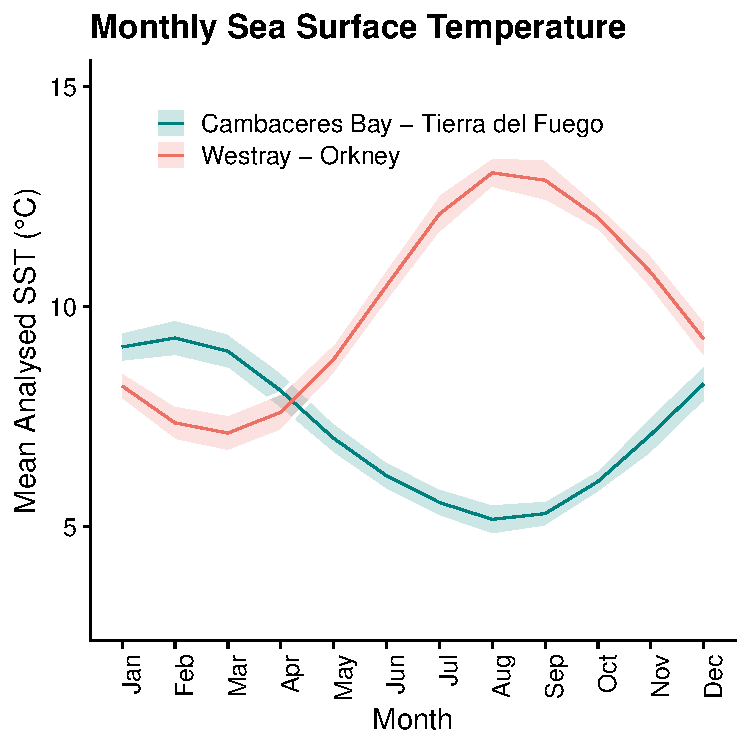
\includegraphics{Manuscript_files/figure-pdf/fig-SSTs-1.pdf}

}

\caption{\label{fig-SSTs}Monthly Sea Surface Temperature values averaged
from years. SST values were sourced from \citet{Good2020-nl}.}

\end{figure}%

We also studied 7 archaeological specimens of \emph{P. vulgata} from the
Quoygrew site on Westray dating to 900 -- 1200 CE. These shells have
previously been studied to characterise seasonal temperature change
during the Medieval Climate Anomaly (810 -- 1229 CE)
\citep{Surge2012-ba}. Together they show a range of lifespans, with some
comparatively long lived for their size (QG1-7246-1, 12 years within 16
mm of growth) making them particularly susceptible to within-shell
time-averaging because of slow growth rates. That said, the majority are
under 5 years old yielding sufficiently fast growth to nearly capture
seasonal amplitudes of SST.

\subsection{Methods}\label{methods}

\subsubsection{Mg/Ca ratios}\label{mgca-ratios}

Mg/Ca elemental imaging was carried out using LIBS at the Leibniz
Zentrum für Archäologie (Mainz-Germany) following previously published
methods \citep{Hausmann2023-ih}. The imaging involves the ablation of
the shell section using an infrared (1064 nm) laser (1--2 mJ, 100 Hz)
onto a surface area of 20--30 µm to generate a plasma plume. This plume
emits light, which is measured using a synchronised spectrometer (delay
time = 0.5 µs, integration time = 1 µs). The resulting light spectrum
quantifies the emission lines of Magnesium (MgII; 279.553 nm) and
Calcium (CaII; 315.887 nm) to determine their intensity ratio. While
these two peaks alone do not represent the molar concentrations of both
elements (as opposed to calibration free LIBS; e.g.
\citep{Martinez-Minchero2022-jz}), the intensity ratio is linearly
correlated to the molar concentration \citep{Hausmann2017-oa} and can be
used as a reliable indicator of Mg/Ca variation within the shell
carbonate. All values reported here are in arbitrary units based on the
ratio of intensities of the peaks above.

Using this system we carried out elemental imaging of the shell
specimens at a resolution of 50--100 µm distance between sampling spots.
Each spot was irradiated 10 times with the 3 first spectra discarded as
a cleaning step and the remaining spectra summed to get an average Mg/Ca
intensity ratio for each sample spot. Subsequently, we re-sampled the
section using a line scan at 10 µm resolution. This leads to an overlap
between sample spots, but also allows for a continuous record without
gaps. Intensity ratios were filtered for cases with high relative
standard deviation (i.e.~more than 10\%). These occurred in places where
the previous sampling procedures for carbonate powder as part of the
oxygen isotope analysis left an uneven sample surface introducing
variability in the plasma generation and thus uncertainty in the data of
these locations.

\subsubsection{Oxygen isotope ratios}\label{oxygen-isotope-ratios}

High-quality \(\delta\)\textsuperscript{18}O values were acquired from
previous publications on \emph{P. vulgata}
\citep{Surge2012-ba, Graniero2017-io}, \emph{N. deaureata} and \emph{N.
magellanica} \citep{Nicastro2020-ih}, in which detailed descriptions of
the stable isotope analysis methodology can be found. In short, all
shells were sectioned along the main growth axis to expose the internal
growth structure. From the exposed section carbonate powder samples were
acquired using a micromill with resolutions of 100--200 µm and by
targeting the calcitic M+2 layer of the shells. Analytical precision of
the isotope values was consistently at 0.05--0.10‰ and values are
reported in per mil units (‰) relative to the VPDB (Vienna Pee Dee
Belemnite) standard.

\begin{figure}

\centering{

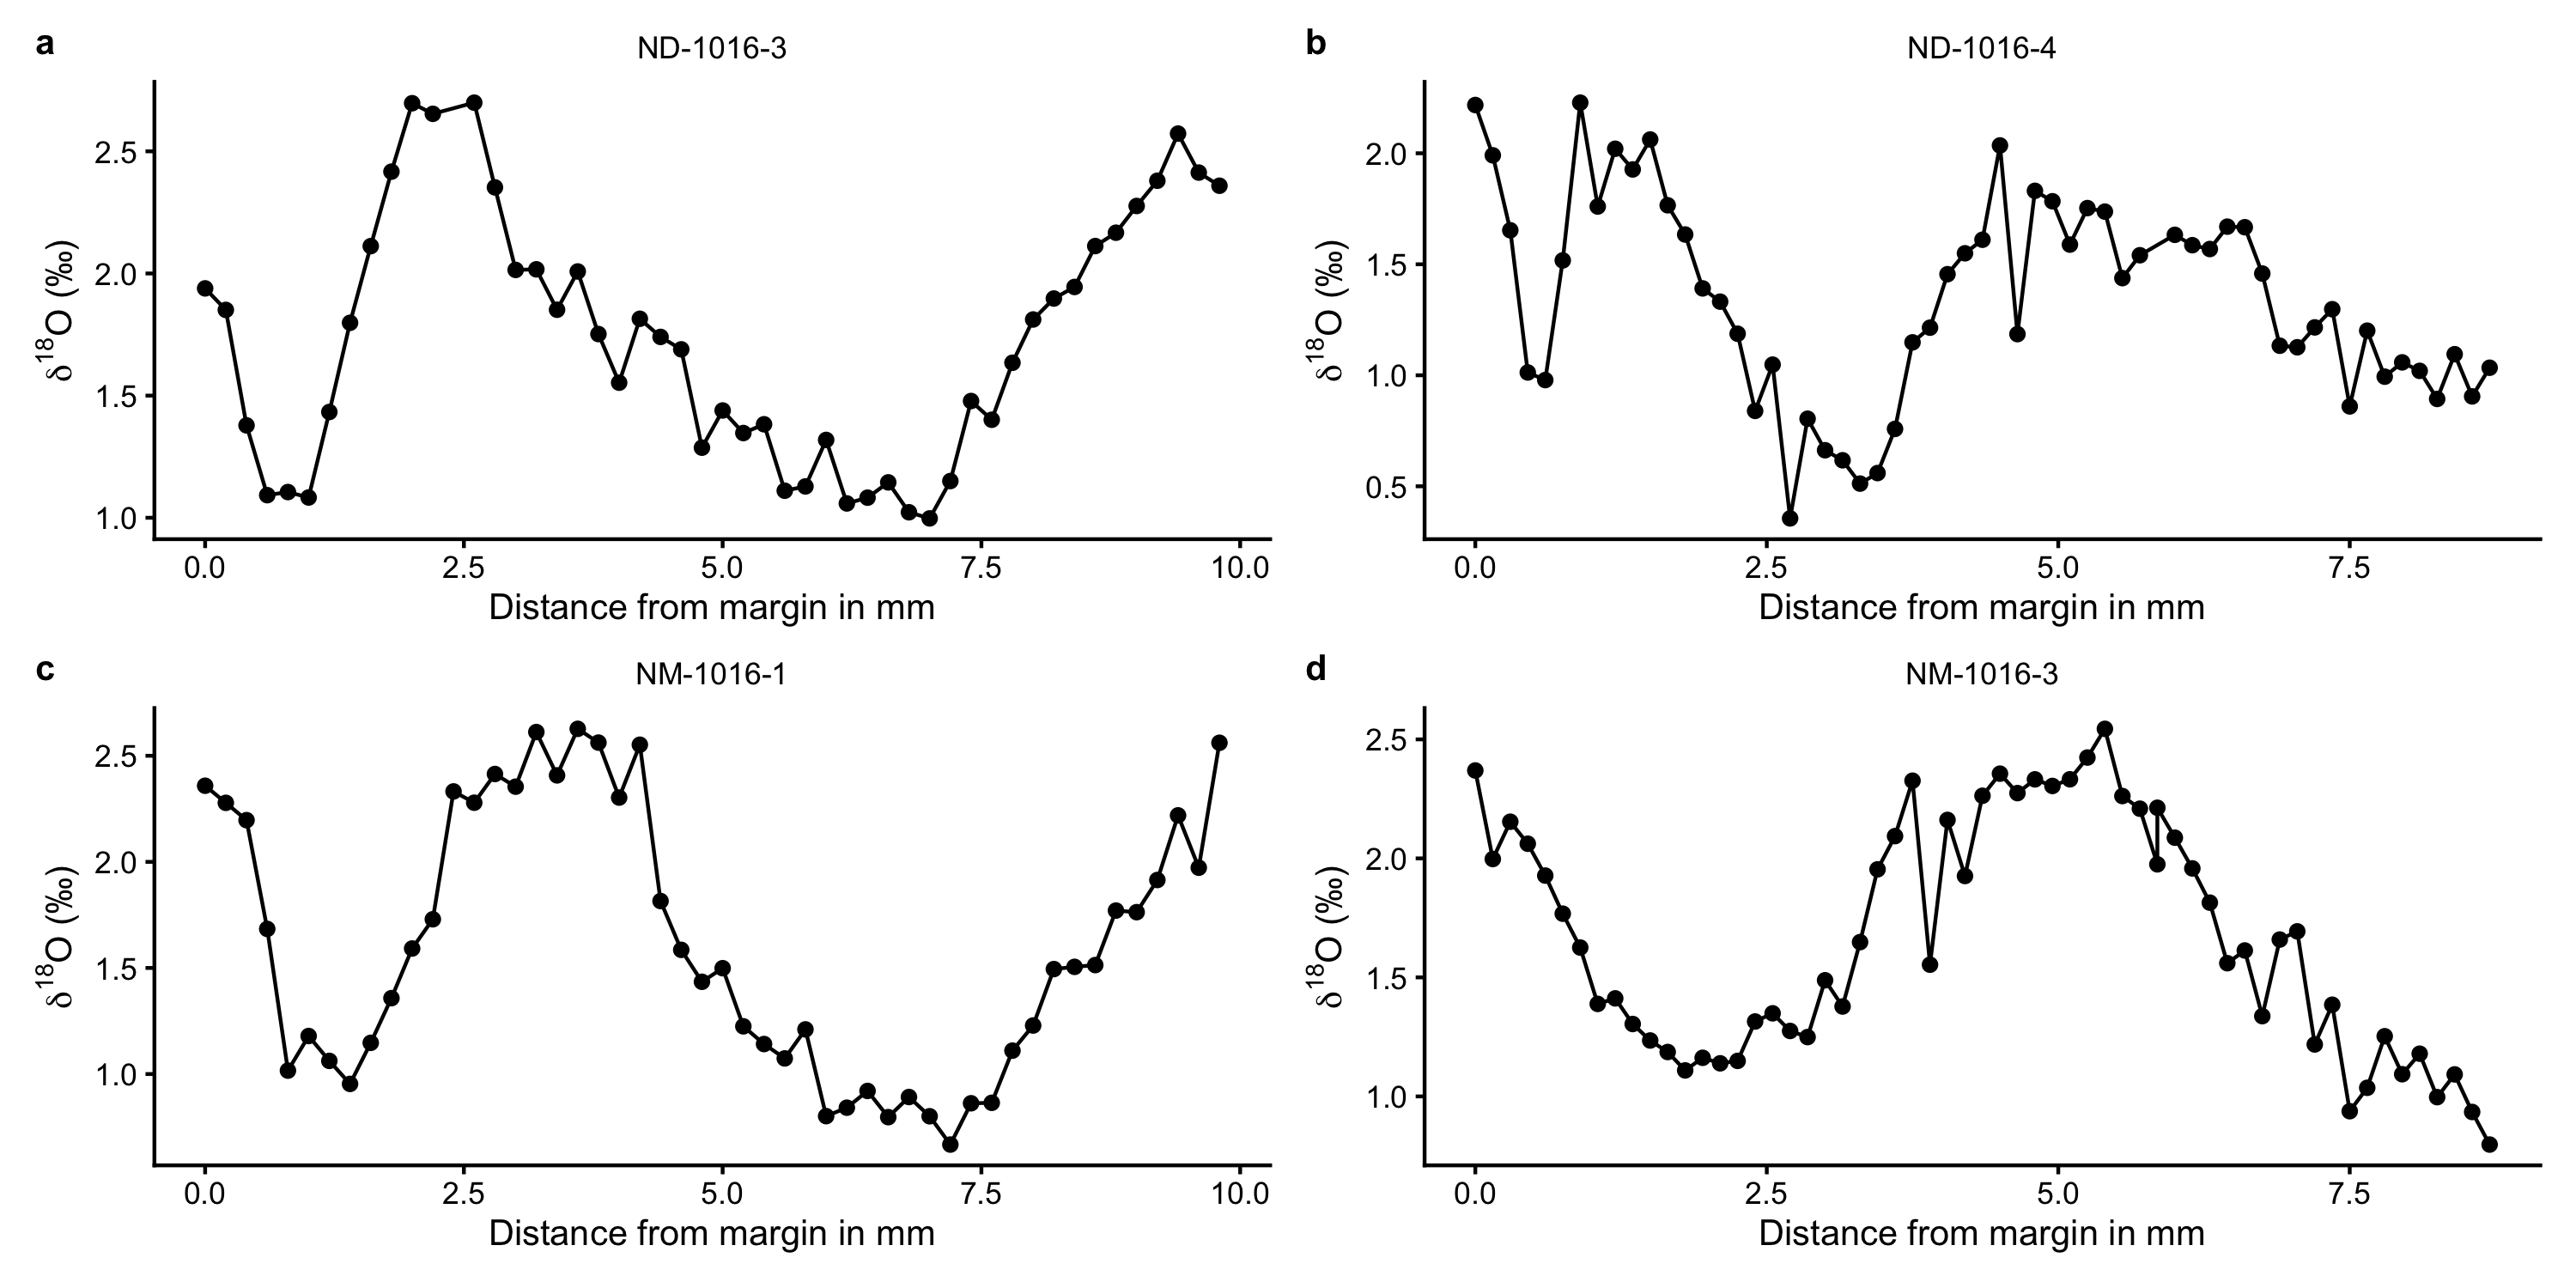
\includegraphics{Manuscript_files/figure-pdf/fig-Nac_iso-1.png}

}

\caption{\label{fig-Nac_iso}Isotope values of \emph{Nacella} sp. limpet
shells from Cambaceres Bay.}

\end{figure}%

Figure~\ref{fig-Nac_iso} and Figure~\ref{fig-Pat_iso} show the
previously acquired sequential \(\delta\)\textsuperscript{18}O-values of
limpet shells by species (\emph{Nacella} sp., and \emph{Patella
vulgata}, respectively. Due to the high sampling resolution, all shells
show seasonally resolved and multi-year quasi-sinusoidal records of SST
change, with \emph{Nacella} sp. shells living 2--3 years and \emph{P.
vulgata} living regularly over 3 years. In those instances where longer
lifetimes are encountered (i.e.~specimen QG1-7246-1,
Figure~\ref{fig-Pat_iso} b) the temporal-resolution is reduced from more
than a dozen of samples per year, to only around 7.

\begin{figure}[H]

\centering{

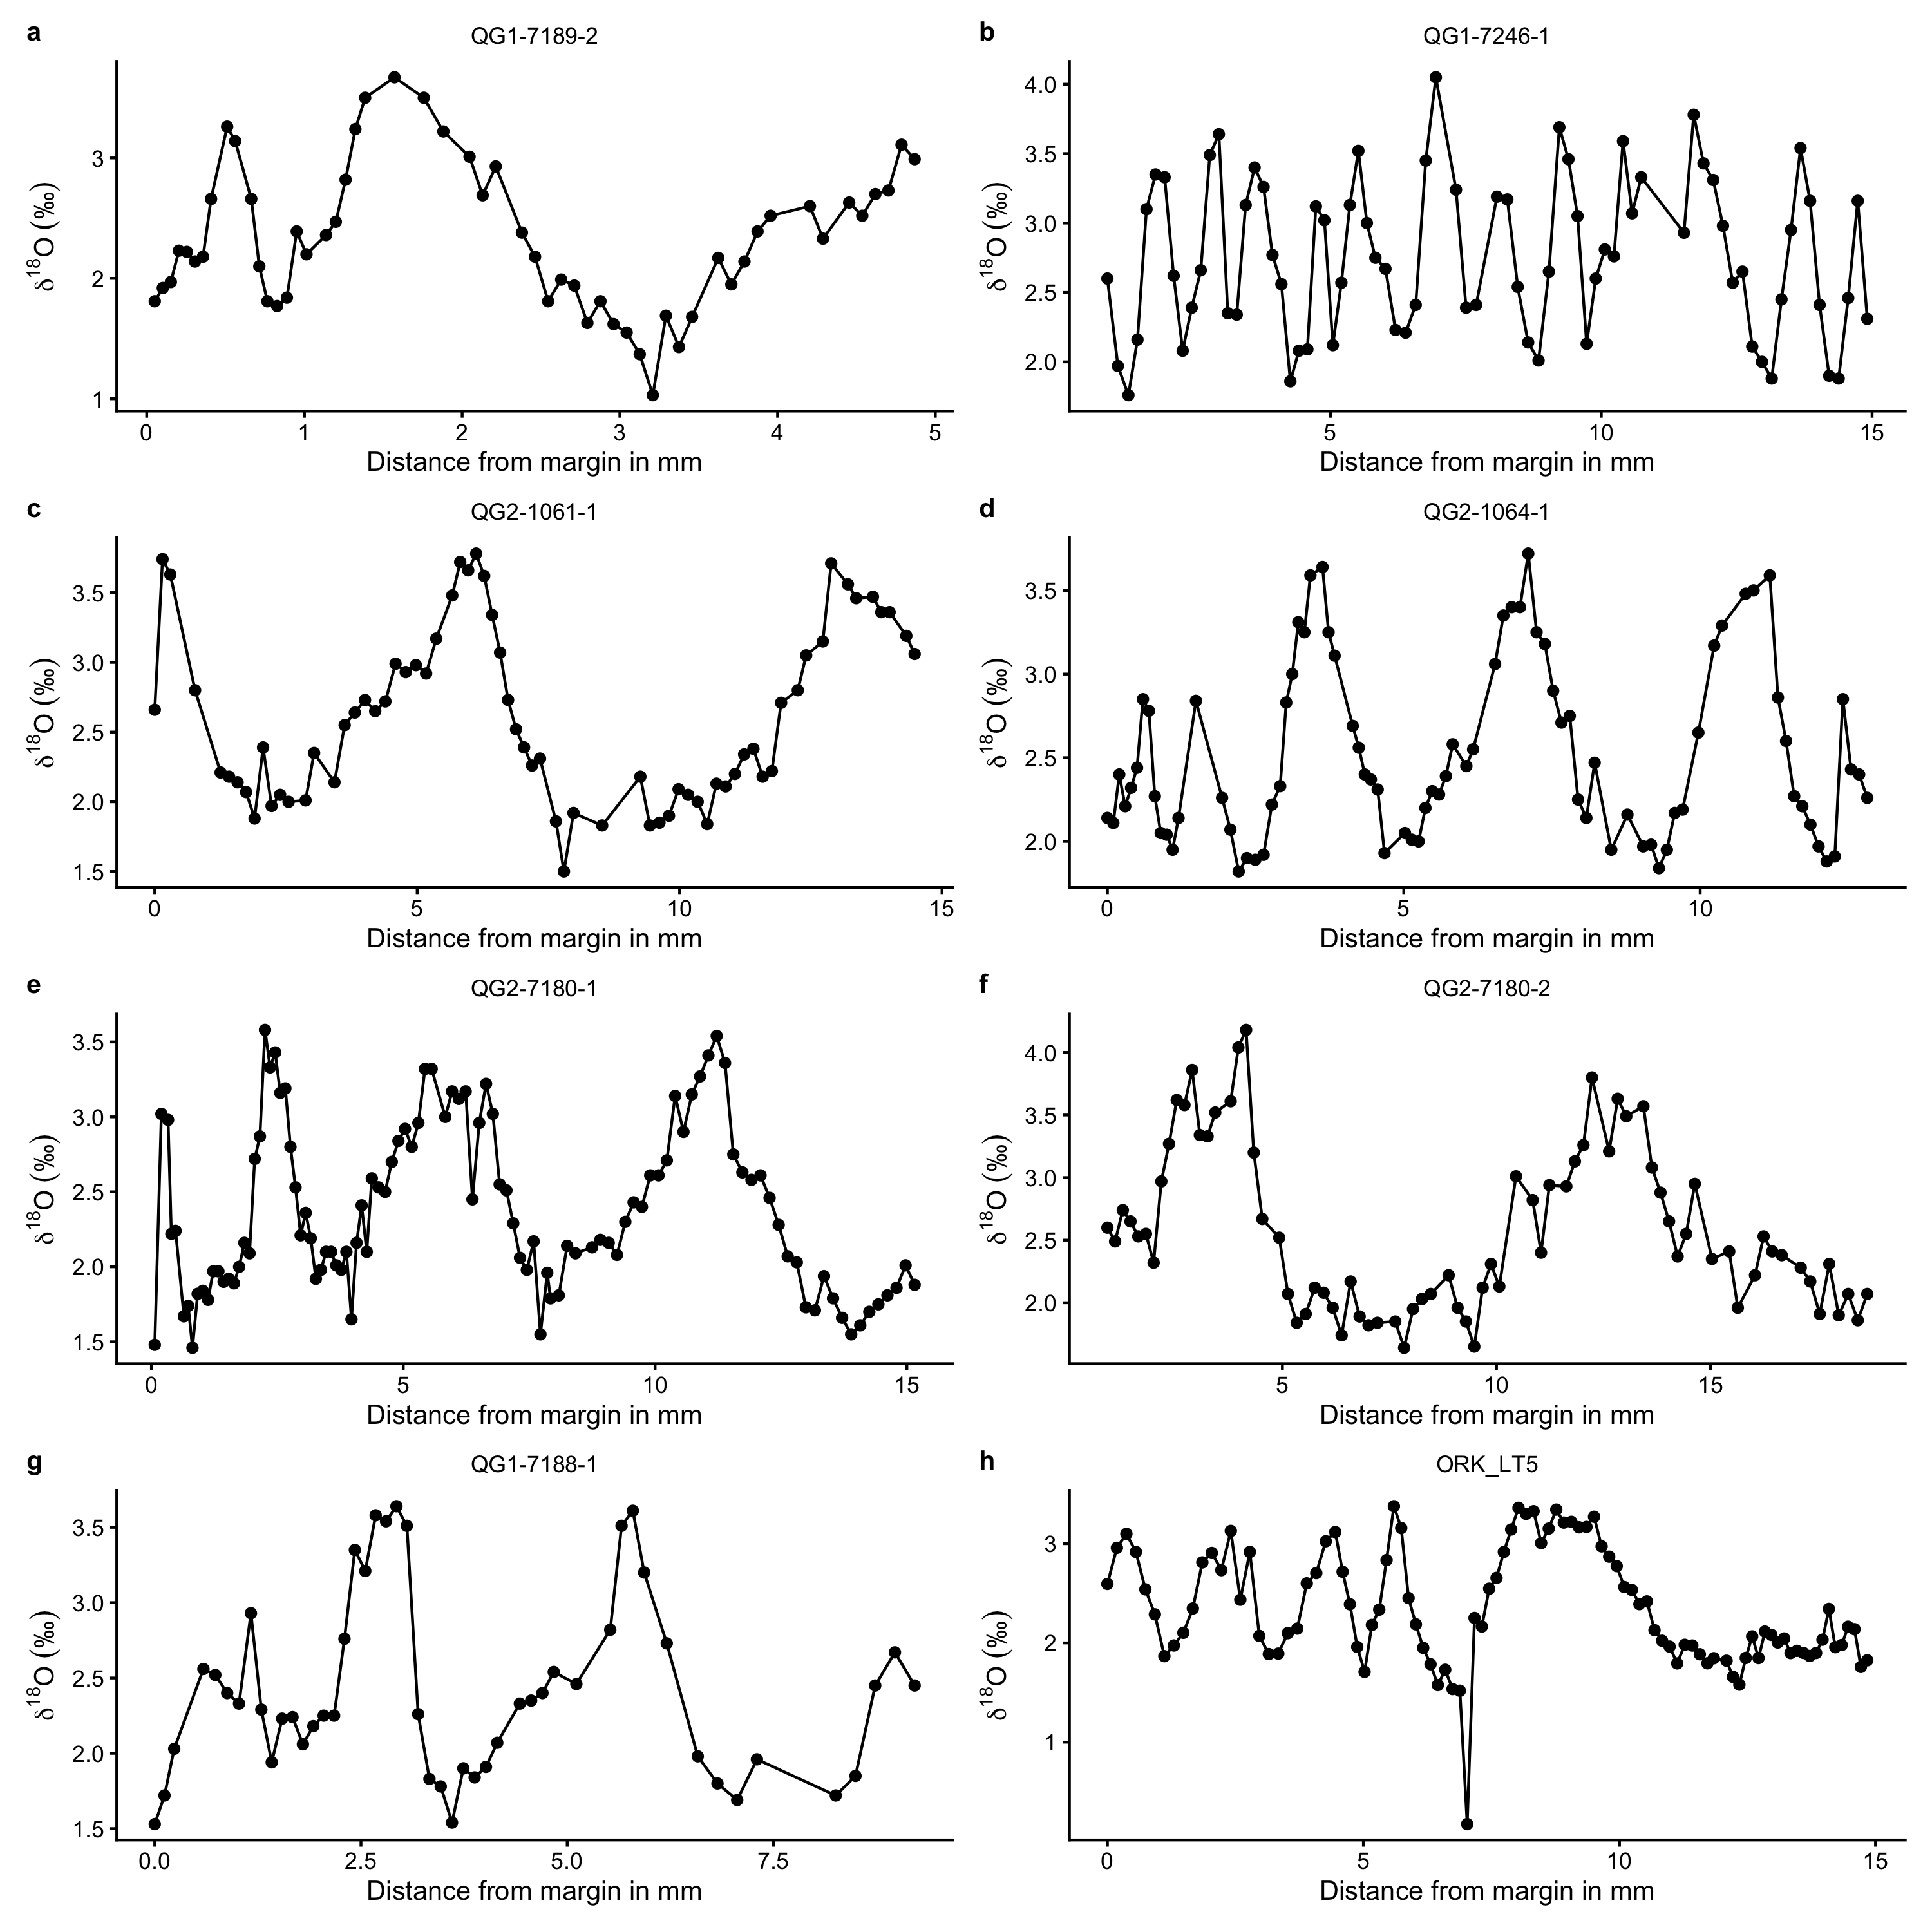
\includegraphics{Manuscript_files/figure-pdf/fig-Pat_iso-1.png}

}

\caption{\label{fig-Pat_iso}Isotope values of \emph{Patella vulgata}
limpet shells from Quoygrew (QG, \emph{a-g}) and Rack Wick Bay (ORK,
\emph{h}) on Westray, Orkney.}

\end{figure}%

\subsection{Dynamic Time Warping}\label{dynamic-time-warping}

Because it is not possible to directly associate the exact sample
locations used in the analysis of stable oxygen isotopes with the LIBS
data, we used dynamic time warping (DTW) to align the time series of
\(\delta\)\textsuperscript{18}O-values and Mg/Ca ratios. DTW is an
algorithm that measures similarity between two proxy-sequences, which
may vary in sampling resolution or interval. By stretching or
compressing sections of the series, DTW finds the probable alignment
between the two sequences. This allows us to compare the proxy data sets
more effectively, ensuring that the temporal dynamics of each shell are
accurately matched despite possible discrepancies in sampling intervals
or rates. We applied the DTW algorithm using the \texttt{dtw} package in
R \citep{Giorgino2009-sj, R_Core_Team2020-mk}, which provides a robust
framework for aligning time series data. This involved selecting
appropriate distance measures and constraints to ensure meaningful
alignment. The process involved iterative adjustments to minimise the
overall distance between corresponding points in the two data sets.

\section{Results}\label{Results}

\subsection{\texorpdfstring{\emph{Patella
vulgata}}{Patella vulgata}}\label{patella-vulgata}

The elemental imaging of \emph{P. vulgata} shells consistently showed
repeating patterns of Mg/Ca intensity ratio changes with high Mg/Ca
intensity ratios indicating and low ratios indicating low temperature
periods. As examples, Figure~\ref{fig-Pat_LIBS} shows the
2D-distribution of elemental ratios across the entire section of ORK-LT5
and the preserved anterior side of QG1-7188-1 (additional maps can be
found in the supplementaries). The repeating patterns are found across
the calcitic layers that are exterior to the myostracum (layers m+2 and
m+3) as well as the layers that are interior (m-2)
\citep{Fenger2007-gf}. The layer m-1, which is also interior, consists
of aragonite and is seen in Figure~\ref{fig-Pat_LIBS} in grey, as its
Mg/Ca intensity ratio consistently falls below the range of interest
(0.2 and above). Compared to other patelloid shells, some of whose
interior is almost entirely made of aragonite, this layer is very thin.
\newline

\begin{figure}[H]

\centering{

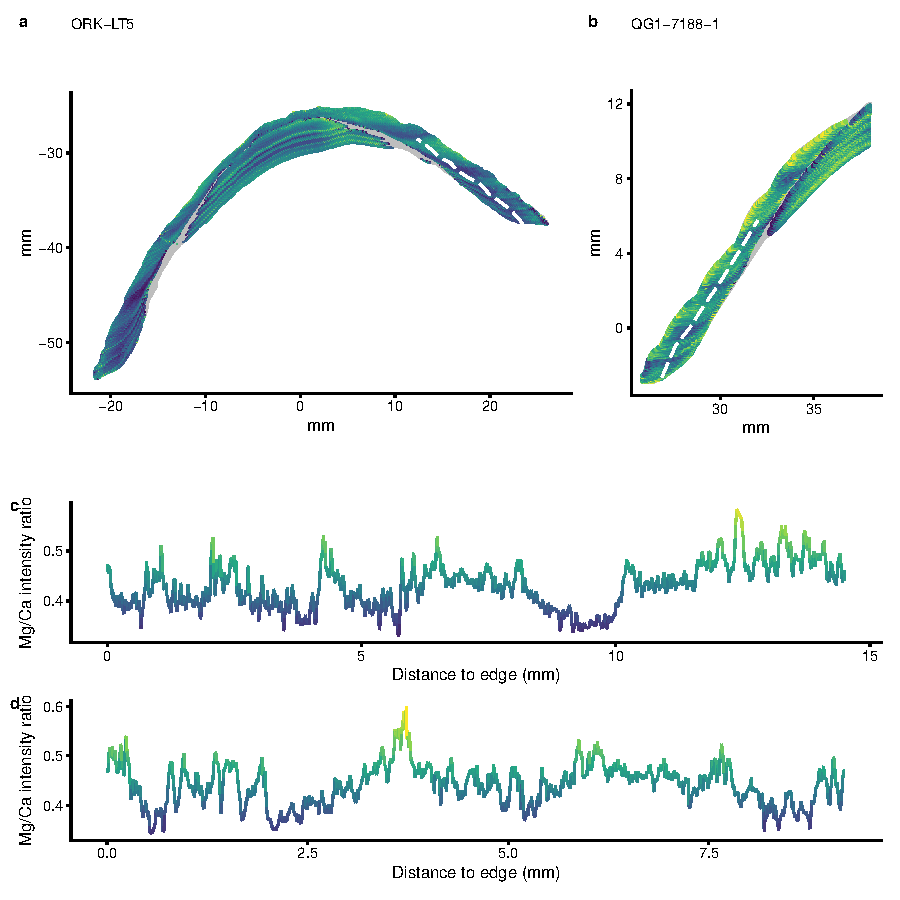
\includegraphics{Manuscript_files/figure-pdf/fig-Pat_LIBS-1.pdf}

}

\caption{\label{fig-Pat_LIBS}Example LIBS maps and line scans of
analysed specimens. (\emph{a+c}) ORK-LT and (\emph{b}+\emph{d})
QG1-7188-1. Note that the ranges of Mg/Ca intensity ratios are not
identical but are chosen arbitrarily to increase contrast. Areas in grey
consist of low-Mg aragonite and fall outside the chosen colour-range.}

\end{figure}%

Both specimens in Figure~\ref{fig-Pat_LIBS} show increased Mg/Ca
intensity ratios towards the outside of the shell and some degree of
intra-increment variability. This is particularly visible in
Figure~\ref{fig-Pat_LIBS} c, where Mg/Ca intensity ratios range from
\textasciitilde0.5--0.7 in the first year of growth (9--12 mm on the
y-axis). A similar pattern is visible in the interior m-2 layer of
ORK-LT5 (Figure~\ref{fig-Pat_LIBS} a), which increase towards the
anterior of the shell (0--10 mm on the x-axis).

Line scans also indicate well the quasi-sinusoidal change of Mg/Ca
intensity ratios expected based on the stable isotope data and
elemental-imaging. That said, some of the variability of Mg/Ca intensity
ratios within one season such as the summer period of QG1-7188-1 between
0.5 and 2.0 mm distance to the shell edge (Figure~\ref{fig-Pat_LIBS} d),
is visible in a more dramatic manner than it appears in the 2D-image,
showing the downside of line-scanning as opposed to the broader milling
approach used for the analysis of carbonate powder
\citep{Ferguson2011-zl}.

Figure~\ref{fig-Pat_Comp} shows the line scan of ORK-LT5 in comparison
to its \(\delta\)\textsuperscript{18}O-values (similar graphs for other
specimen can be found in the supplementaries). The measurements of the
distance to the shell edge are not entirely identical, most likely
because one growth increment can have a range of distances to the edge,
depending on where one measures, and a line scan along the interior
would be shorter than a line scan along the exterior. That said,
increases and decreases of both proxies seem to mirror each other and to
be well aligned.

\begin{figure}

\centering{

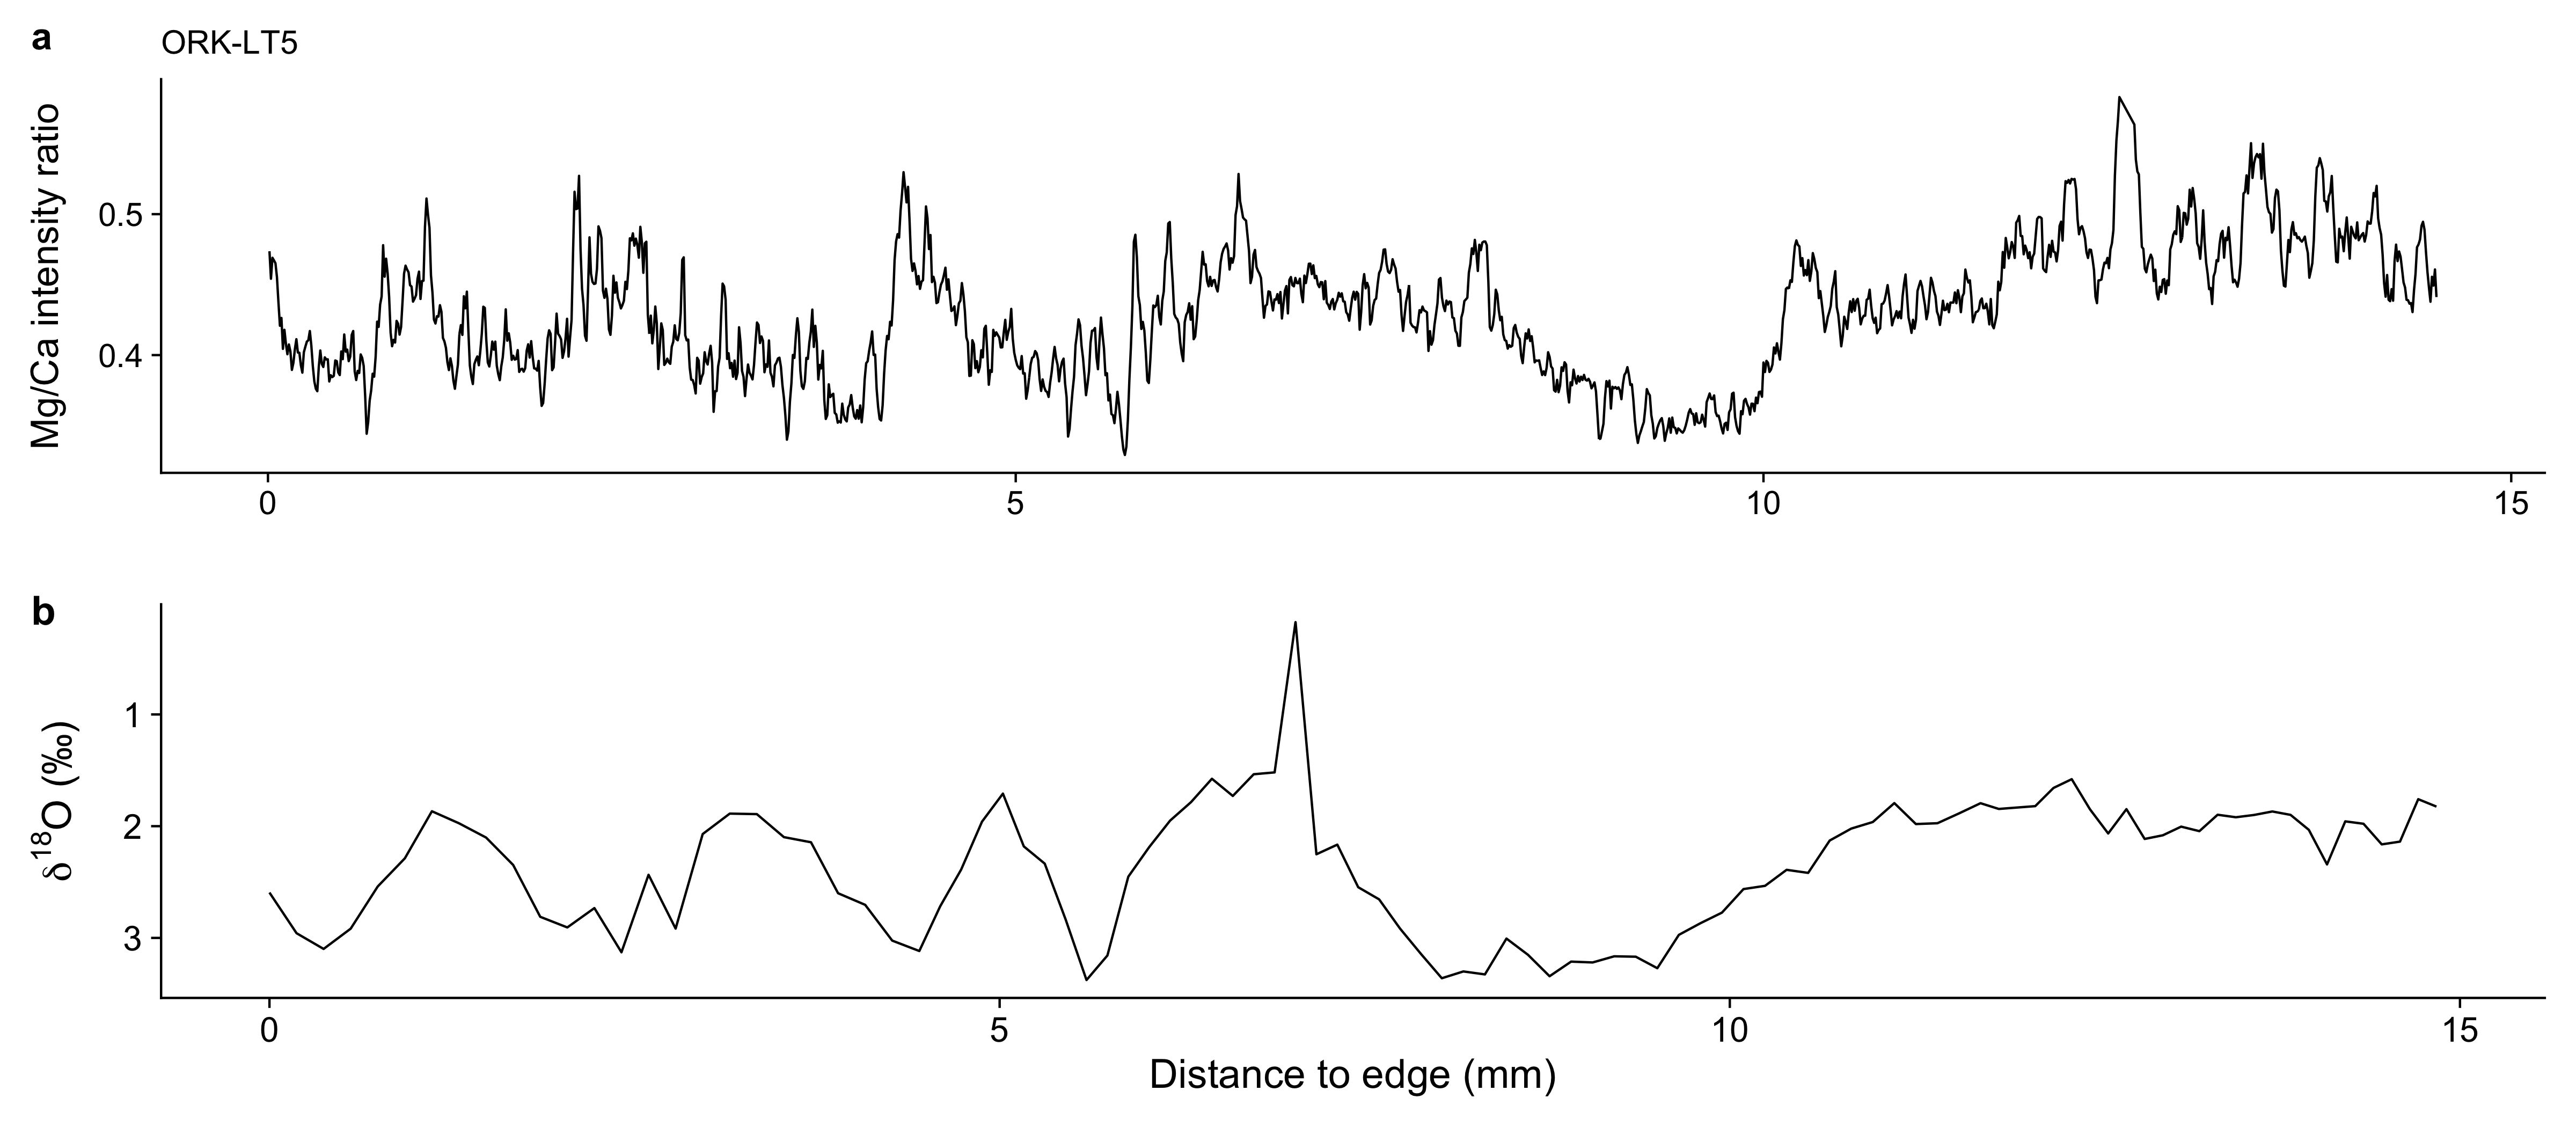
\includegraphics{Manuscript_files/figure-pdf/fig-Pat_Comp-1.png}

}

\caption{\label{fig-Pat_Comp}Comparison of LIBS line-scan and sequential
\(\delta\)\textsuperscript{18}O-values of specimen ORK-LT5}

\end{figure}%

Aligning the records programmatically using dynamic time warping,
allowed us to compare them directly to determine specimen-specific
equations and quantify the correlation of both proxies
(Figure~\ref{fig-Pat_Corr}). The equations for all specimens are
different but the majority (barring one: QG1-7246-1) do seem to cluster
around shared parameters (\(\delta\)\textsuperscript{18}Ο = 0.6 -- 0.065
* Mg/Ca). The various coefficients of determination
(R\textsuperscript{2}) range between 0.81 (QG1-7246-1) and 0.95
(QG1-7189-2). These specimens are also the oldest and youngest
specimens, respectively, suggesting that lower growth rates and time
averaging had a negative effect on the correlation of both proxies. The
mean R\textsuperscript{2} value of the individual \emph{P. vulgata}
specimens is 0.89, suggesting a generally good fit between the two
proxies.

\begin{figure}

\centering{

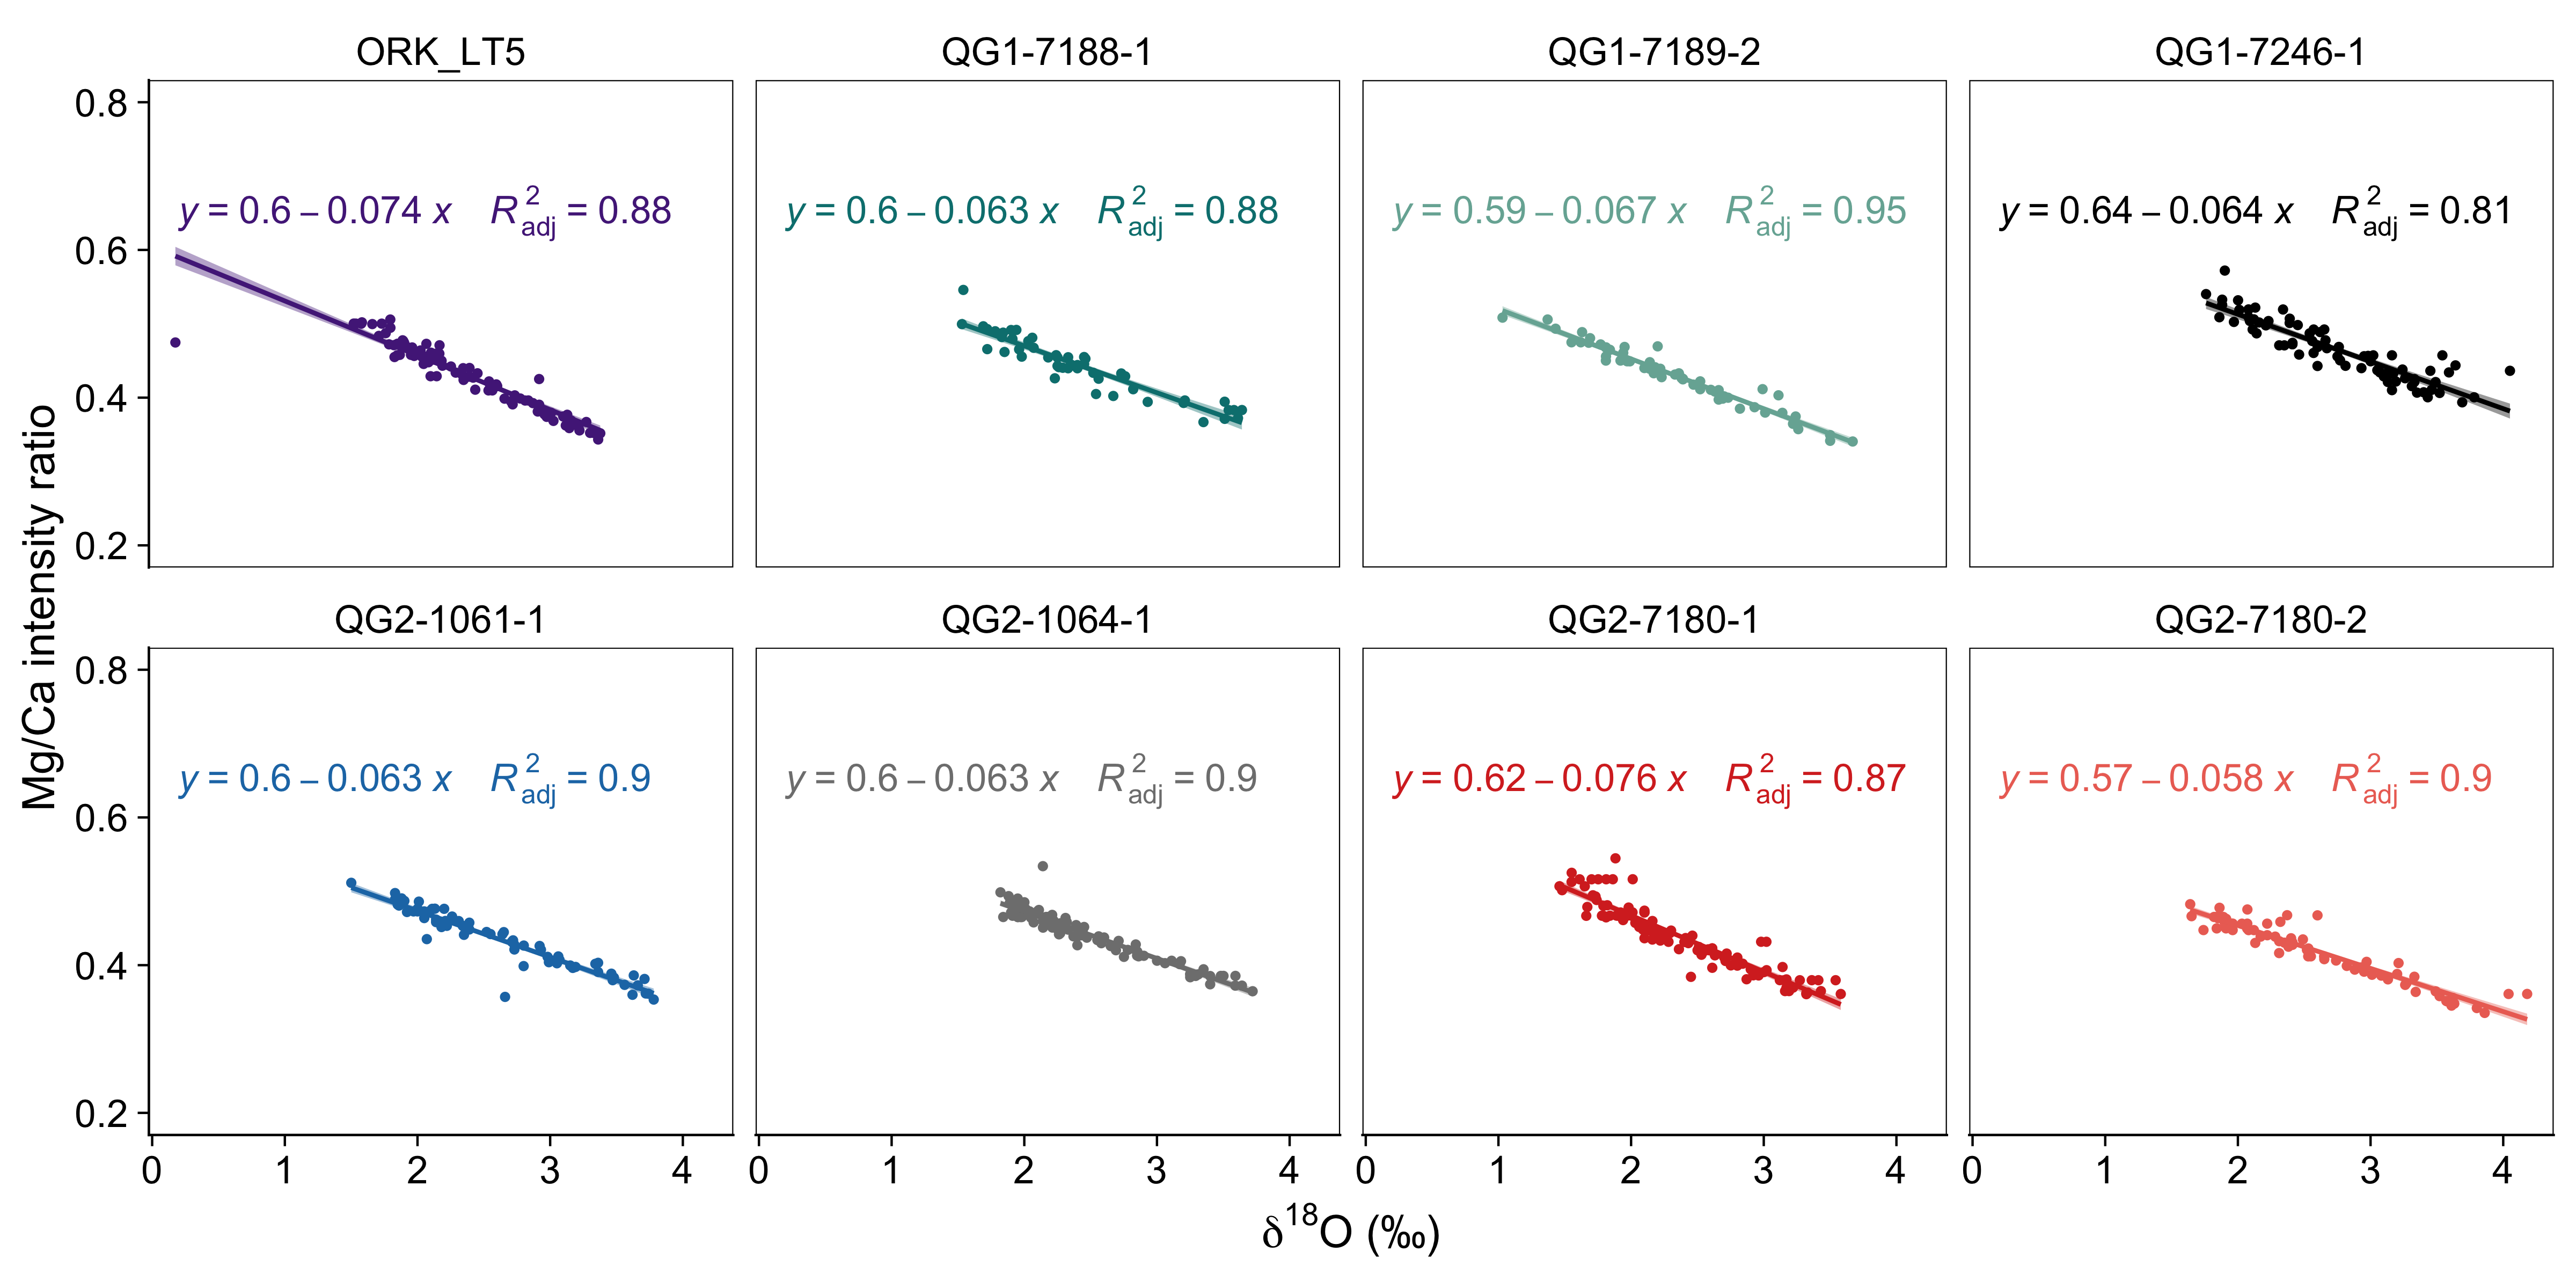
\includegraphics{Manuscript_files/figure-pdf/fig-Pat_Corr-1.png}

}

\caption{\label{fig-Pat_Corr}Correlation graphs for \emph{Patella
vulgata} specimens.}

\end{figure}%

\subsection{\texorpdfstring{\emph{Nacella}
sp.}{Nacella sp.}}\label{nacella-sp.}

The LIBS data for \emph{Nacella} sp. specimens is less straightforward
with shells being much thinner and thus patterns being more difficult to
make out. Both specimens (ND-1016-3 and NM-1016-3) shown as example in
Figure~\ref{fig-Nac_LIBS} (see additional graphs in supplementaries)
also experience increases of Mg/Ca intensity ratio towards the exterior
of the shell, similar to the \emph{P. vulgata} specimens from Orkney.
This intra-increment heterogeneity combined with the thinness of the
shell, further complicates their analysis compared to \emph{P. vulgata}
or other \emph{Patella} species \citep{Hausmann2019-fi}. Nevertheless,
repeating patterns were visible in the anterior section of the shell,
which were also mirrored in the inner layers (m-2) of specimens
NM-1016-3 (Figure~\ref{fig-Nac_LIBS} b).

\begin{figure}[H]

\centering{

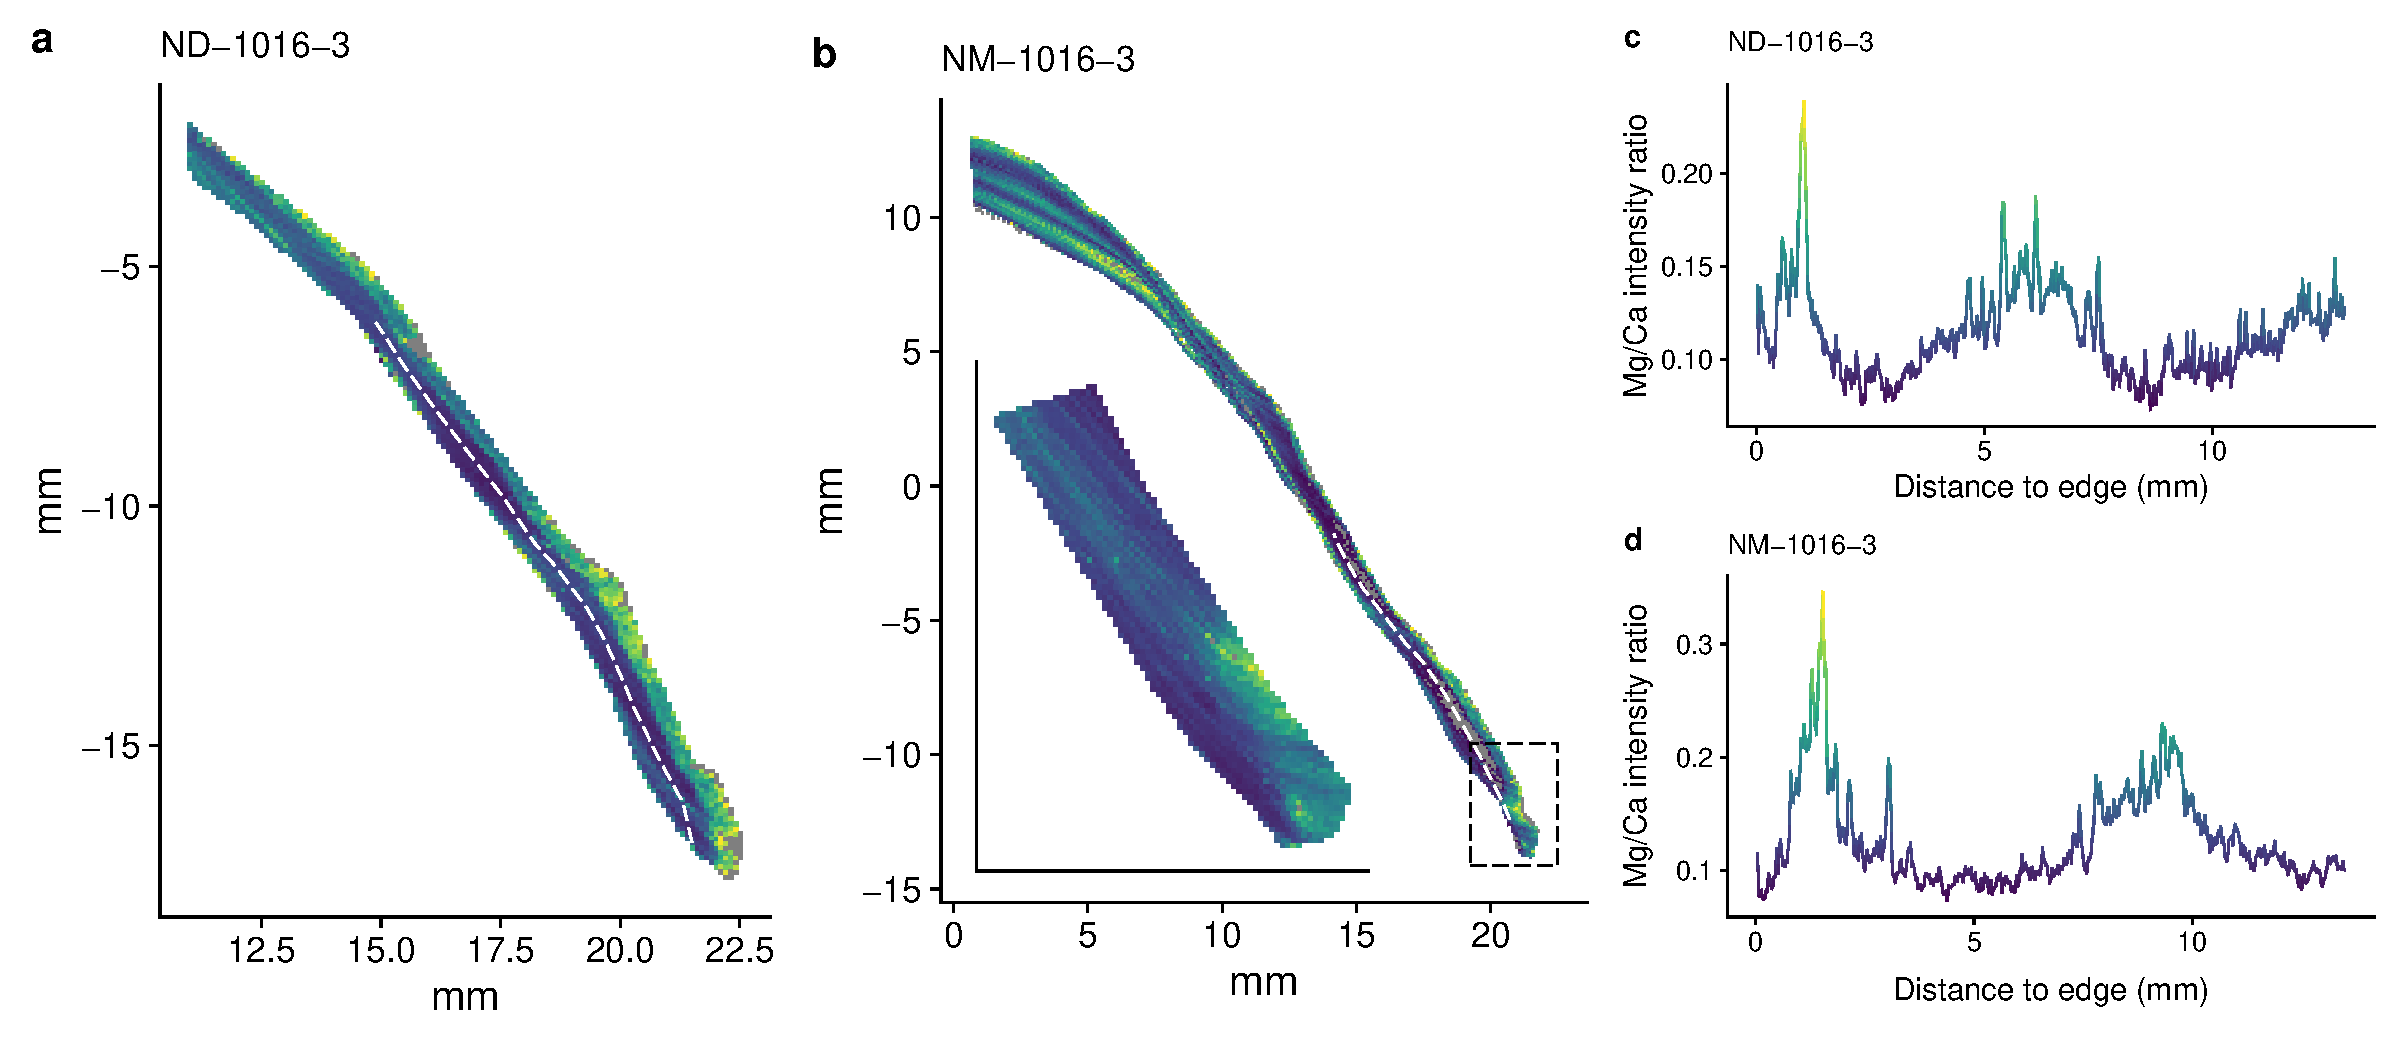
\includegraphics{Manuscript_files/figure-pdf/fig-Nac_LIBS-1.pdf}

}

\caption{\label{fig-Nac_LIBS}Example LIBS maps and line scans of
analysed \emph{Nacella} sp. specimens. (\emph{a+c}) ND-1016-3 and
(\emph{b}+\emph{d}) NM-1016-3. Note that the ranges of Mg/Ca intensity
ratios are not identical but are chosen arbitrarily to increase
contrast. Areas in grey consist of low-Mg aragonite and fall outside the
chosen colour-range. Note the inset in (\emph{c}) where the shell edge
has been resampled using a higher resolution (50 µm instead of 100 µm)
to better understand the Mg/Ca ratios at the shell edge.}

\end{figure}%

Interestingly, the Mg/Ca intensity ratios in the \emph{Nacella} sp.
shells were much lower (0.05--0.30) than those seen in other patelloid
species (e.g.~0.3--0.7 in \emph{Patella vulgata} above, or 0.5--1.5 in
Hausmann \emph{et al}. \citeyearpar{Hausmann2023-ih}) using the same
emission lines. While the intensity ratio depends chiefly on the chosen
emission lines to calculate the proportion of the chosen Magnesium to
the chosen Calcium peak, the low ratios still indicate lower
concentrations than seen elsewhere, or seen only in aragonitic parts of
e.g.~\emph{Patella} shells. Similar observations have been made before
\citep{Graniero2017-io}. Strong intra-increment heterogeneities are
visible along the exterior of the shells (m+3 layer), where Mg/Ca
intensity ratios are higher, particularly in specimen ND-1016-3
(Figure~\ref{fig-Nac_LIBS}). The step from lower to higher along the
increment is not gradual, as is the case in NM-1016-3 (see inset of
Figure~\ref{fig-Nac_LIBS} b), but rather step-wise. Sampling across this
boundary in a linear scan would most likely lead to erroneous results.
Also sampling across gradual changes as in NM-1016-3 can influence the
overall correlation graph for a specimen.

Line scans reflect well the changes previously indicated by
\(\delta\)\textsuperscript{18}O values and also indicate about two years
of recorded growth. That said, the 2D imaging suggests that in both
specimens a third summer can be added to the total record, which is not
captured by the line scans.

Figure~\ref{fig-Nac_Comp} shows the line scans of ND-1016-3 and
NM-1016-3 in comparison to their \(\delta\)\textsuperscript{18}O-values
(similar graphs for the other \emph{Nacella} sp. specimen can be found
in the supplementaries). Compared to the \emph{P. vulgata} records,
these mirror each other much more clearly, due to the brief period
recorded in the shells and its simple make-up.

\begin{figure}

\centering{

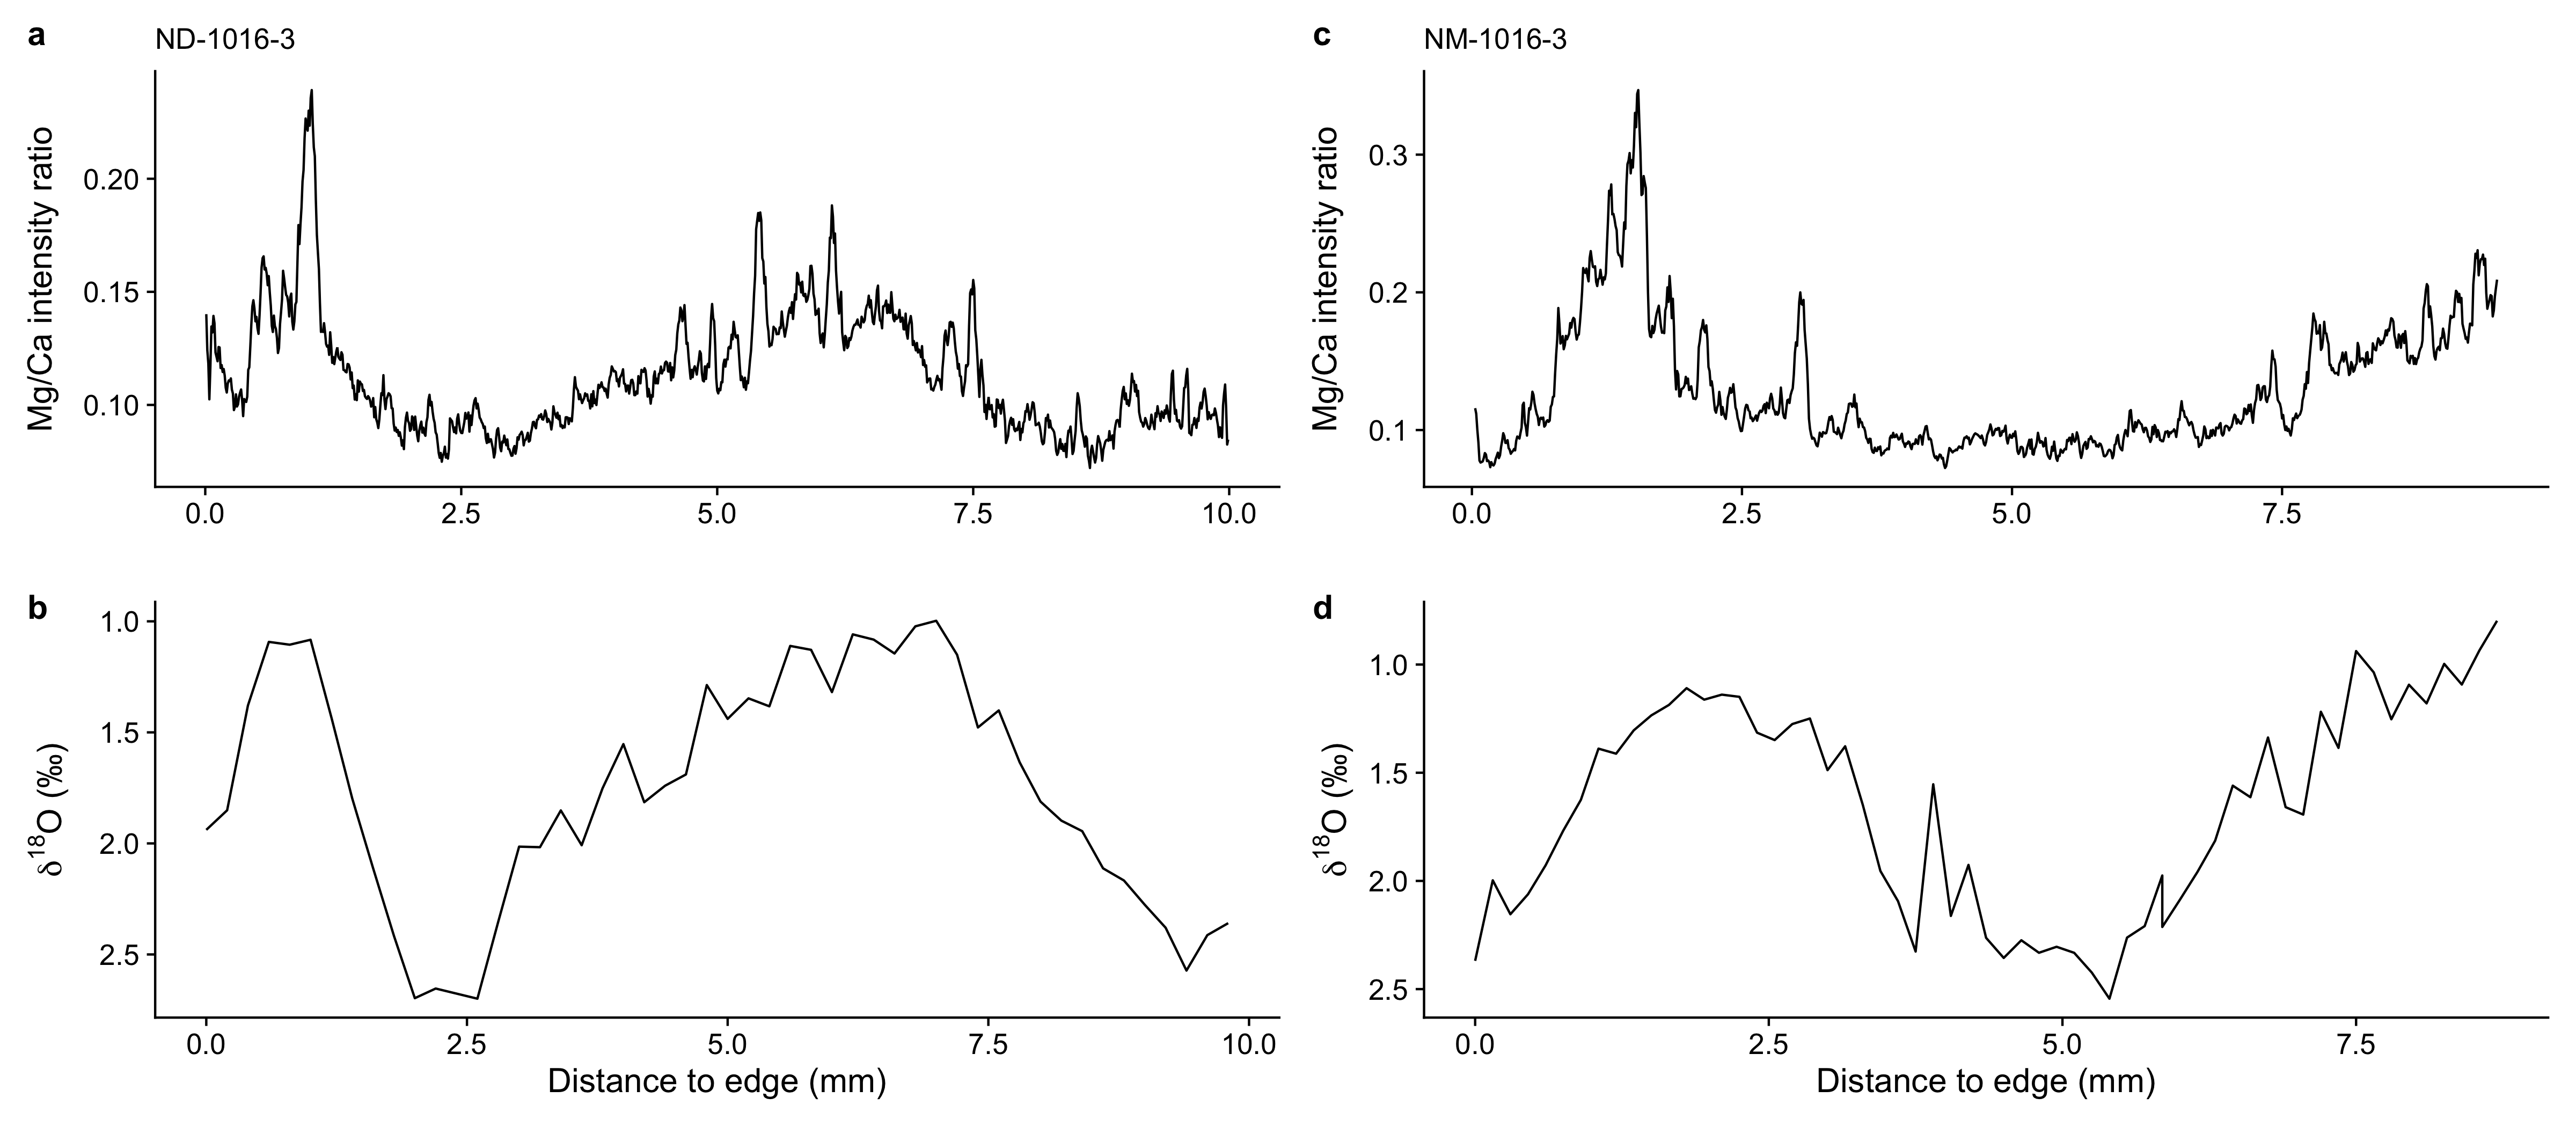
\includegraphics{Manuscript_files/figure-pdf/fig-Nac_Comp-1.png}

}

\caption{\label{fig-Nac_Comp}Comparison of LIBS line-scan and sequential
\(\delta\)\textsuperscript{18}O-values of \emph{Nacella} sp. specimens.}

\end{figure}%

The \emph{Nacella} sp. specimens showed similarly clustered
correlations, which interestingly were not grouped by species. In fact,
specimens ND-1016-3 (\emph{Nacella deaureata)} and NM-1016-3
(\emph{Nacella magellanica}) are almost identical in their fitted
equations (Figure~\ref{fig-Nac_Corr}). Both also share a high
coefficient of determination (R\textsuperscript{2}) of 0.95 and 0.92
respectively, with the remaining specimens being somewhat lower
(R\textsuperscript{2} = 0.76 for ND-1016-4 and R\textsuperscript{2}=0.84
for NM-1016-3). The mean R\textsuperscript{2} value for each
\emph{Nacella} species is 0.86 for \emph{Nacella deaureata} and 0.88 for
\emph{Nacella magellanica}. Why two specimens of different species are
so well aligned is not entirely certain and randomness cannot for now be
ruled out. That said, since they both have a high R\textsuperscript{2}
value, it might just be that they were both minimally affected by
factors other than SST, including the sampling location of our line
scans.

\begin{figure}

\centering{

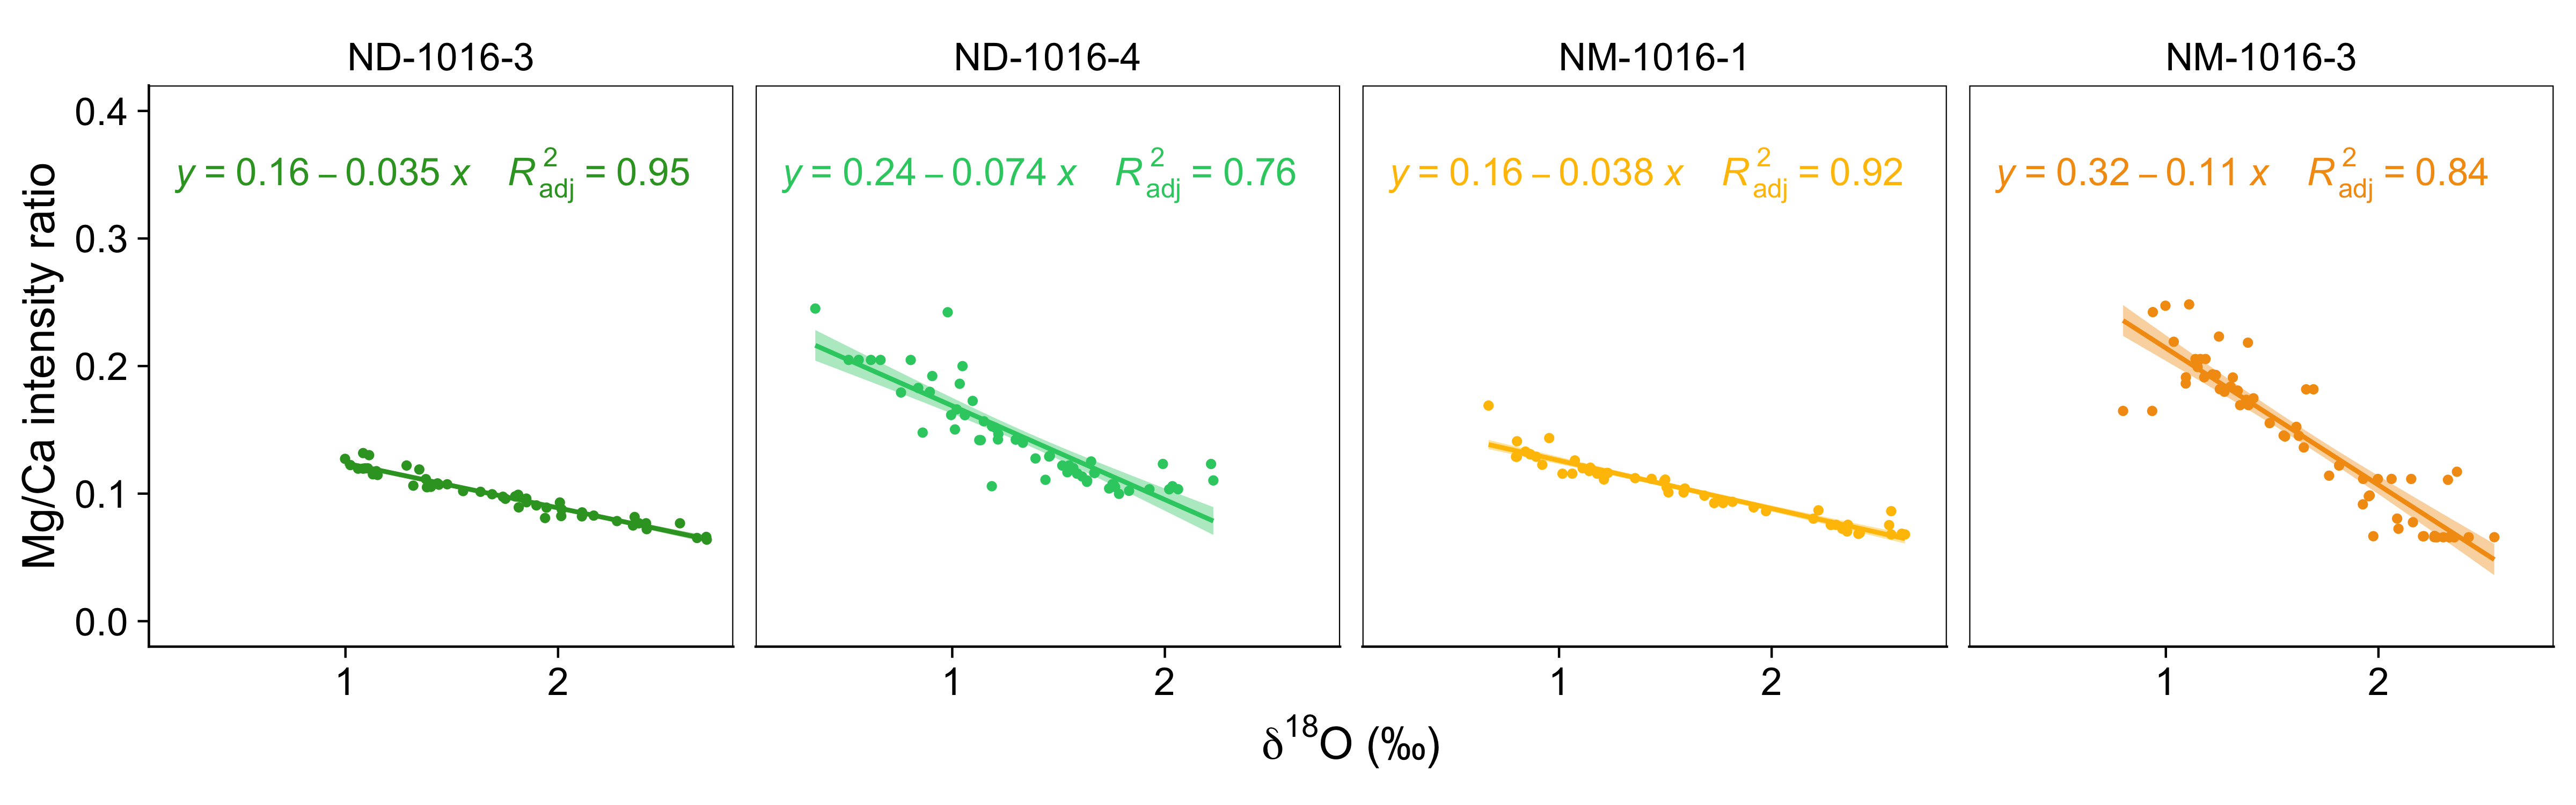
\includegraphics{Manuscript_files/figure-pdf/fig-Nac_Corr-1.png}

}

\caption{\label{fig-Nac_Corr}Correlation graphs for \emph{Nacella} sp.
specimens}

\end{figure}%

\section{Discussion}\label{Discussion}

The Mg/Ca ratios from the 2D elemental imaging present positive results
on SST being the main factor behind Mg/Ca concentration in three
Atlantic limpet species. Annually repeating patterns of increasing
(spring/summer) and decreasing (autum/winter) SST were also visible in
the line scans, albeit less straightforward than in the 2D-data.
Nevertheless, the resulting R\textsuperscript{2}-values for each species
were high (\emph{P. vulgata mean R\textsuperscript{2}}=0.89, \emph{N.
deaureata mean R\textsuperscript{2}}=0.86\emph{, N. magellanica mean
R\textsuperscript{2}}=0.88). These results are similar to previously
published data on \emph{Patella} sp. shells (Table
\hyperref[Table_2]{2}): R\textsuperscript{2} values of \emph{P.
depressa} lie between 0.78 and 0.87 \citep{Garcia-Escarzaga2021-ij}, for
\emph{P. caerulea} from the Mediterranean between 0.78 and 0.96 ---
barring one outlier of 0.33 (specimen MP64A), which had increased Mg/Ca
ratios in increments with rich organic contents \citep{Hausmann2019-fi}.

\phantomsection\label{Table_2}
\fontsize{8pt}{8pt}\selectfont

\begin{longtable}[]{@{}
  >{\raggedright\arraybackslash}p{(\columnwidth - 8\tabcolsep) * \real{0.1250}}
  >{\raggedright\arraybackslash}p{(\columnwidth - 8\tabcolsep) * \real{0.1562}}
  >{\raggedright\arraybackslash}p{(\columnwidth - 8\tabcolsep) * \real{0.1094}}
  >{\raggedright\arraybackslash}p{(\columnwidth - 8\tabcolsep) * \real{0.2031}}
  >{\raggedright\arraybackslash}p{(\columnwidth - 8\tabcolsep) * \real{0.4062}}@{}}
\caption{Correlations of Mg/Ca with \(\delta\)\textsuperscript{18}O and
SST found in other studies. Bold R\textsuperscript{2} values are
interpreted as outliers. * indicates that only SST data and no other
geochemical data was used. ** these samples were used to determine a
shared R\textsuperscript{2}-value of 0.79.}\tabularnewline
\toprule\noalign{}
\begin{minipage}[b]{\linewidth}\raggedright
Species
\end{minipage} & \begin{minipage}[b]{\linewidth}\raggedright
Locality
\end{minipage} & \begin{minipage}[b]{\linewidth}\raggedright
Specimen
\end{minipage} & \begin{minipage}[b]{\linewidth}\raggedright
R\textsuperscript{2}
\end{minipage} & \begin{minipage}[b]{\linewidth}\raggedright
Study
\end{minipage} \\
\midrule\noalign{}
\endfirsthead
\toprule\noalign{}
\begin{minipage}[b]{\linewidth}\raggedright
Species
\end{minipage} & \begin{minipage}[b]{\linewidth}\raggedright
Locality
\end{minipage} & \begin{minipage}[b]{\linewidth}\raggedright
Specimen
\end{minipage} & \begin{minipage}[b]{\linewidth}\raggedright
R\textsuperscript{2}
\end{minipage} & \begin{minipage}[b]{\linewidth}\raggedright
Study
\end{minipage} \\
\midrule\noalign{}
\endhead
\bottomrule\noalign{}
\endlastfoot
\emph{P. depressa} & Northern Spain & LAN541 & 0.87 &
\citep{Garcia-Escarzaga2021-ij} \\
& & LAN545 & 0.86 & \\
& & LAN554 & 0.78 & \\
& & LAN559 & 0.82 & \\
\emph{P. caerulea} & Croatia & ISTPC1 & 0.9 & \citep{Hausmann2019-fi} \\
& & ISTPC2 & 0.84 & \\
& Crete & AF1911A & 0.91 & \\
& & AF3003A & 0.92 & \\
& Israel & AKKPC2 & 0.96 & \\
& & AKKPC3 & 0.89 & \\
& & FRMPC1 & 0.84 & \\
& & FRMPC2 & 0.96 & \\
& Libya & MO31A & 0.83 & \\
& & \textbf{MP64A} & \textbf{0.33} & \\
& & MP67A & 0.96 & \\
& & MP68A & 0.81 & \\
& Malta & MA10 & 0.82 & \\
& Tunisia & TUNPC1 & 0.81 & \\
& & TUNPC2 & 0.78 & \\
& Turkey & ANTPC1 & 0.95 & \\
& & ANTPC2 & 0.93 & \\
& & KIZPC1 & 0.94 & \\
& & KIZPC2 & 0.86 & \\
\emph{P. rustica} & Gibraltar & \textbf{JL1} & \textbf{0.02} &
\citep{Ferguson2011-zl} \\
& & JL2 & 0.8** & \\
\emph{P. caerulea} & Gibraltar & JM00 & 0.69** & \\
& & JM30 & 0.83** & \\
\emph{P. vulgata} & Orkney & ORK-LT5 & not reported, here 0.88 &
\citep{Graniero2017-io} and this study \\
\end{longtable}

\normalsize

\emph{P. rustica} has two studied specimens (JL1 and JL2) with
R\textsuperscript{2}-values of 0.02 and 0.8, respectively
\citep{Ferguson2011-zl} (Figure~\ref{fig-Ferg}). Together with the data
from two \emph{P. caerulea} shells (JM00 and JM30 with
R\textsuperscript{2}-values of 0.69 and 0.83), the data from JL2 was
used determine a general Mg/Ca-SST relationship with an
R\textsuperscript{2}-value of 0.79. JL1 was disregarded in that
calculation, as well as the second year of growth in JM00, which
produced anomalous data. While no additional information about those
specimens is available, it seems likely that discarded the Mg/Ca ratios
from JM00, which were interpreted as an ontogenetic trend, were
potentially influenced by the same intra-increment heterogeneity we see
in some of our shell specimens as well. Since these shells were analysed
by homogenising the carbonate powder of the m+2 layer and the more
exterior m+3 layer, these heterogeneities could potentially increased
the Mg/Ca ratio unpredictably, leading to what might look like an
ontogenetic trend in a linear dataset. Whether these anomalies affected
JL1 in the same way, albeit stronger, is not clear but it might well be
possible.

\begin{figure}

\centering{

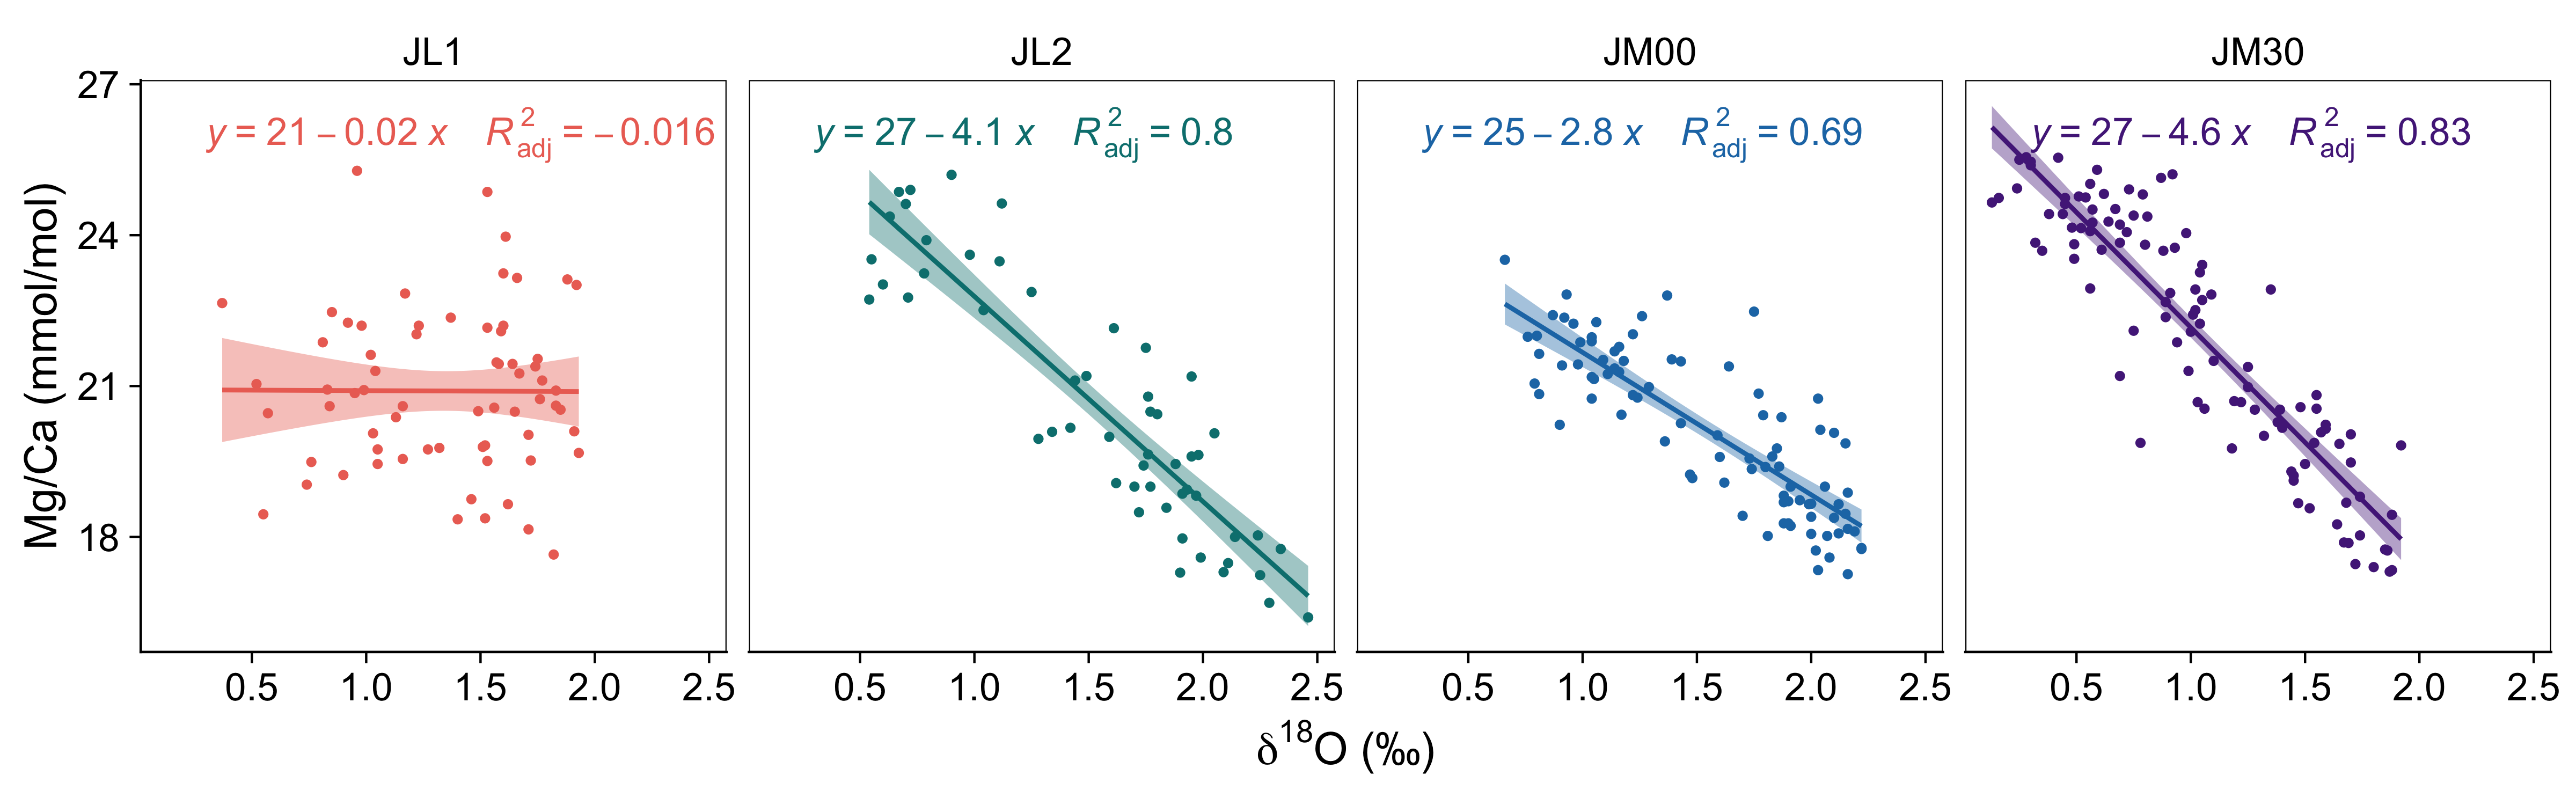
\includegraphics{Manuscript_files/figure-pdf/fig-Ferg-1.png}

}

\caption{\label{fig-Ferg}Correlation graphs for Ferguson et al., (2011)
specimens.}

\end{figure}%

Another shell whose results we aim to explain further is ORK-LT5, which
has previously been shown to have no substantial correlation with
\(\delta\)\textsuperscript{18}O or SST in implication
\citep{Graniero2017-io}. Different to other specimens of this study, we
were able to resample this specimen and to acquire Mg/Ca data on a
slightly higher resolution (20--30 µm spots in a 100 µm raster compared
to 50 µm spots spaced at 150--300 µm) and using 2 dimensions, as well as
using a continuous high-resolution line-scan at (20--30 µm spots spaced
at 10 µm) (Figure~\ref{fig-ORK_sub}). These additional data revealed
previously missed summer peaks at around 2--3 mm distance to the shell
edge (grey box in Figure~\ref{fig-ORK_sub}) and revealed additional
growth at the very edge (dashed box in Figure~\ref{fig-ORK_sub})
mirroring the change towards warmer temperatures at the time of
collection (August). Including these missing parts lead to a better
alignment of both records and a resulting R\textsuperscript{2}-value of
0.88 (Figure~\ref{fig-ORK_sub}).

\begin{figure}

\centering{

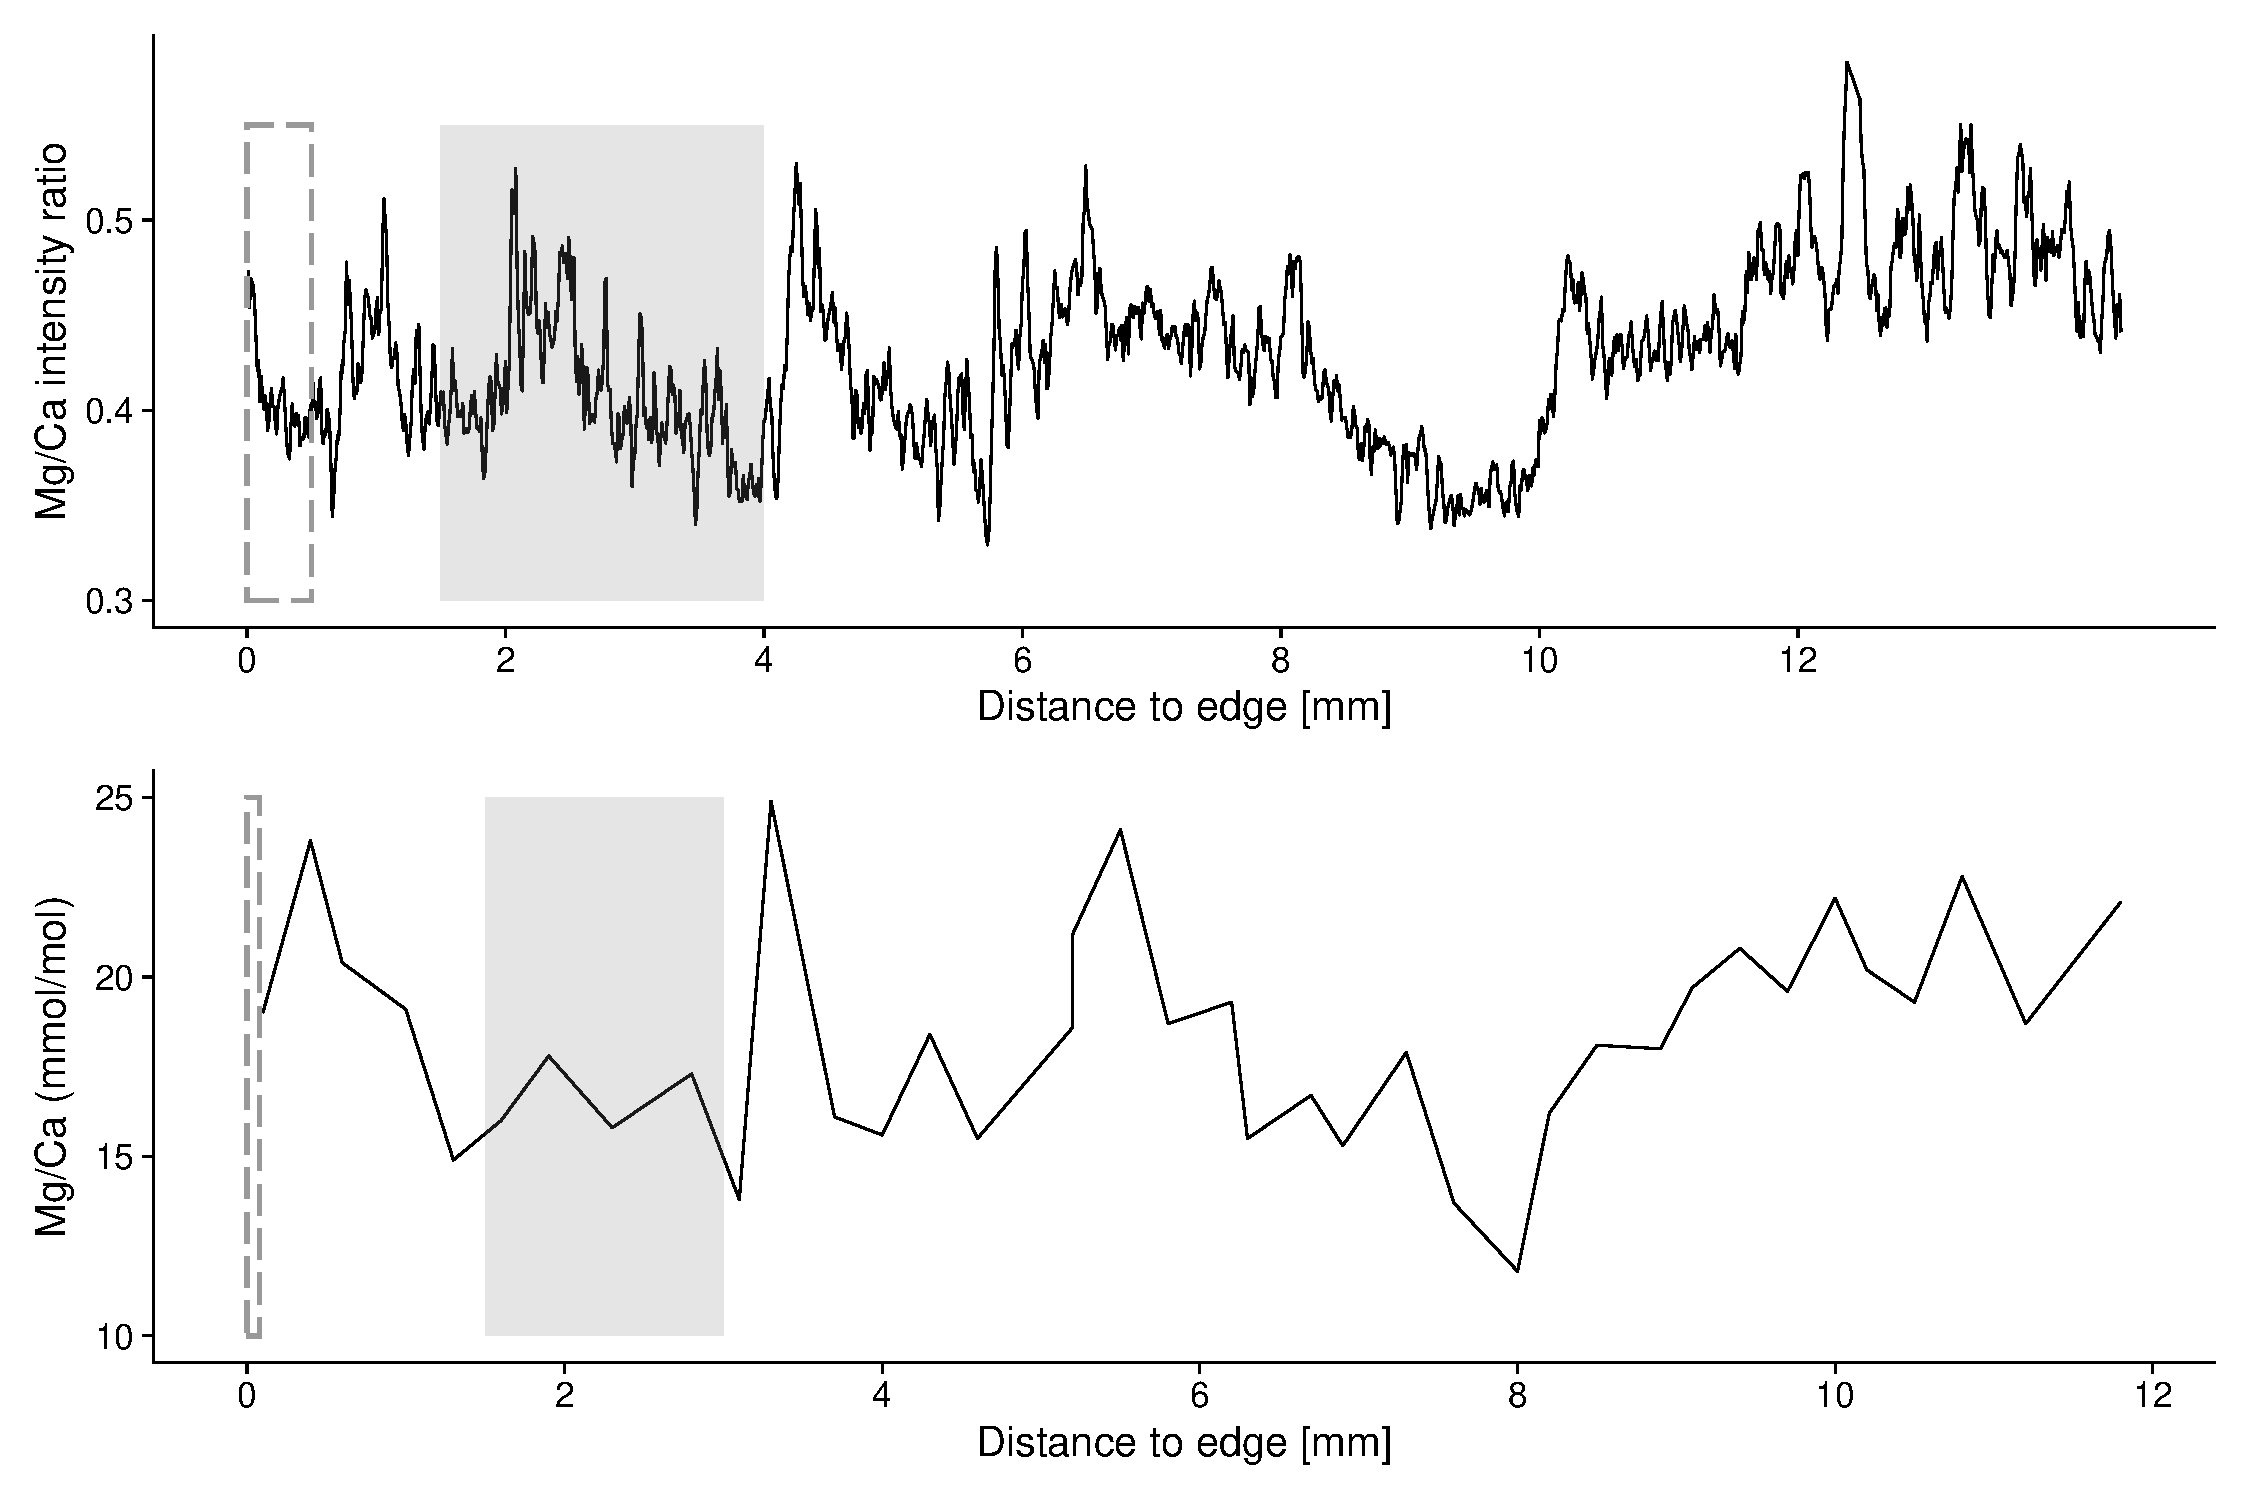
\includegraphics{Manuscript_files/figure-pdf/fig-ORK_sub-1.pdf}

}

\caption{\label{fig-ORK_sub}Comparison of previous and new Mg/Ca data
for ORK-LT5 explaining the previously unsuccessful correlation of Mg/Ca
and \(\delta\)\textsuperscript{18}O-values}

\end{figure}%

We were not able to resample the \emph{Nacella} sp. specimens in
Graniero \emph{et al.} \citeyearpar{Graniero2017-io}, which had
similarly unrelated records of \(\delta\)\textsuperscript{18}O and Mg/Ca
and pointed to no relationship between elemental ratios and SST at all.
However, we were able to source other modern specimens of the same
species from Tierra del Fuego, which shall serve here as an indicator.
Similar to other patelloid shells, the results of the \emph{Nacella}
specimens in our study were successful with high
R\textsuperscript{2}-values (0.76--0.95) and suggest Mg/Ca as a reliable
proxy for SST (Figure~\ref{fig-Nac_Comp} and supplementaries). Why these
results are different from the studied \emph{Nacella} sp. specimens in
Graniero \emph{et al}. \citeyearpar{Graniero2017-io} is not obvious, but
the occasional alignment of the Mg/Ca and
\(\delta\)\textsuperscript{18}O records of their shells (Figure 6 in
Graniero \emph{et al}. \citeyearpar{Graniero2017-io}) indicate that
there is some relationship that --- potentially due to the low sampling
resolution or intra-increment heterogeneity --- is not perfectly
visible, leading to an overall result of an uncorrelated relationship
between Mg/Ca and SST.

\section{Conclusion}\label{conclusion}

This study presents high-resolution and 2D information on Mg/Ca
concentrations in modern and archaeological patelloid shells and their
relationship to sea surface temperature. The results for \emph{Patella
vulgata}, \emph{Nacella deaureata}, and \emph{Nacella magellanica} were
consistently promising with mean R\textsuperscript{2}-values of 0.89,
0.86, and 0.88 respectively.

LIBS elemental imaging provided some insight into elemental anomalies
found particulary in the external parts (m+3 layer) of the shell, which
introduce intra-incremental heterogeneity and which cannot be reconciled
with modern SST changes or SST changes recorded in the
\(\delta\)\textsuperscript{18}O of the same shells. Our 2D approach
allowed us to avoid these areas of intra-increment heterogeneity and
focus on areas that are predominantly controlled by changes in SST.

These results are particularly promising for future analyses of
patelloid shells for the study of season of collection in archaeological
sites as well as the reconstruction of sub-annual climatic conditions in
the past. Shells of the species studied here are widely available along
the European Atlantic façade and the Argentinian coastline and make up a
significant part of marine mollusc remains in archaeological sites of
those regions
\citep{Colonese2011-ab, Villagran2011-ld, Zangrando2016-yl}. Improving
their analysis in terms of cost and time efficiency through the benefits
of LIBS, which can be used in this context as a screening tool for
targeted \(\delta\)\textsuperscript{18}O analysis focusing on annual
minima and maxima revealed in the Mg/Ca record, will allow researchers
to increase sample numbers and produce larger and more in-depth climatic
studies than previously possible.


\renewcommand\refname{References}
  \bibliography{bibliography.bib}


\end{document}
